\chapter{HiFiLES: an open source GPU-powered, High-Order Large-Eddy Simulation code}
\chaptermark{HiFiLES: open source High-Order, LES code}

%Describe the history, structure, and capabilities of HiFiLES. Compile data from the 2014 AIAA paper.

%\subsection{History}
%Mention the work of the original SD++ developers and initial intention.
%
%Describe the process of transforming an academic code into an open source code that could be developed by the academic community at large.
%
%Describe differences between HiFiLES and other open source high-order codes, including PyFR.
%
%\subsection{Structure}
%Design decisions and object-oriented programming. 
%
%Describe the classes present in the code (even though the foundations of the code were developed by previous lab members, the developers' guide and readability has been improved by current lab members).
%
%Data structures and GPU/CPU implementation. Place references to Castonguay's and Williams's theses.
%
%\subsection{Capabilities}
%Point to all publications that contain results from HiFiLES/SD++
%
%Large-Eddy Simulation developments. Point to research by Lodato and Bull.

% !TEX root = ./thesis.tex

\section{Introduction}

During the last decade, the \gls{acl} of the Department of Aeronautics and Astronautics at Stanford University has developed a series of high-order numerical schemes and computational tools that have demonstrated the viability of this technique. In this chapter, the code named \gls{hf}, developed in the \gls{acl} and built on top of SD++ (Castonguay et al.\cite{castonguay2011}), is described in detail with a particular emphasis on robustness in a range of applications and \gls{vv}. \gls{hf} takes advantage of the synergies between applied mathematics, aerospace engineering, and computer science in order to achieve the ultimate goal of developing an advanced high-fidelity simulation environment.

In addition to the original characteristics of the SD++ code, \gls{hf} includes some important physical models and computational methods such as: \gls{les} using explicit filters and advanced \gls{sgs} models, high-order stabilization techniques, shock detection and capturing for compressible flow calculations, and local time stepping.

During the development of this software, several key decisions have been taken to guarantee a flexible and lasting infrastructure for industrial Computational Fluid Dynamics simulations:
\begin{itemize}
\item The selection of the \gls{esfr} scheme on unstructured grids\cite{vincent2011new}. The flexibility of this method has been critical to guarantee a correct solution independently of the particular physical characteristics of the problem.
\item High performance, materialized in a multi-\gls{gpu} implementation that takes advantage of the ease of parallelization afforded by discontinuous solution representation. Furthermore, \gls{hf} aims to guarantee compatibility with future vector machines and revolutionary hardware technologies.
\item Code portability by using ANSI C++ and relying on widely-available, and well-supported mathematical libraries like Blas, LAPACK, CuBLAS, and ParMetis.
\item Object oriented structure to boost the re-usability and encapsulation of the code. This abstraction enables modifications without incorrectly affecting other portions of the code. Although some level of performance is traded for re-usability and encapsulation, the loss in performance is minor.
\end{itemize}

As the mathematical basis and computational implementation of \gls{hf} have been described in previous work~\cite{castonguay2011}, the goal of this chapter is to illustrate the level of robustness of \gls{hf} for interesting problems. This will be accomplished via a \gls{vv} study, which is fundamental for increasing the credibility of this technology in a competitive industrial framework.

In particular, to ensure that the implementation of the aforementioned features in \gls{hf} is correct, the following verification tests are shown: checks of spatial and temporal order of accuracy using the \gls{mms} in 2D and 3D for viscous and inviscid flows and characterization of stable time-step limits. After the Verification, a detailed Validation of the code is presented to illustrate that the solutions provided by \gls{hf} are an accurate representation of the real world. Simulations of complex flows are validated against experimental or \gls{dns} results for the following cases: laminar flat-plane, flow around a circular cylinder, SD7003 wing-section and airfoil at 4$\degr$ angle of attack, the Taylor-Green Vortex, and \gls{les} of a square cylinder.

The organization of this chapter is as follows. Section~\ref{sec:govEq} provides a description of the governing equations. Section~\ref{sec:numerics} describes the mathematical and numerical algorithms implemented in the code. Section~\ref{sec:verification} focuses on the \gls{vv} of \gls{hf}, and the conclusions are summarized in Section~\ref{sec:conclusion_hf}. It is important to highlight that the contents of this chapter mirror the \gls{aiaa} paper\cite{lopez2014verification} created jointly with members of the \gls{acl} and Francisco Palacios.


% !TEX root = ./main.tex

\section{Governing Equations}
\label{sec:govEq}
\subsection{Navier Stokes equations}

The \gls{ns}~\cite{Landau1993} equations provide a complete (dynamical) description of a viscous fluid and expresses the conservation of mass, momentum and energy. The complete system of equations (without source terms and assuming adiabatic boundary conditions at the solid wall) can be written in the following conservative form:

\begin{equation}\label{ns}
\frac{\partial U}{\partial t} +  \nabla \cdot {\bf F} = 0
\end{equation}

where ${\bf F} = (F,G,H) = (F_I,G_I,H_I) - (F_V,G_V,H_V)$ and
\begin{equation}
U = \l(
\begin{tabular}{c}
$\rho$\\
$\rho u$\\
$\rho v$\\
$\rho w$\\
$\rho e$
\end{tabular}
\r) 
\end{equation}
\begin{equation}
F_I = \l(
\begin{tabular}{c}
$\rho u$\\
$\rho u^2 + p$\\
$\rho uv$\\
$\rho uw$\\
$\rho ue + pu$
\end{tabular}
\r) \;\; 
G_I = \l(
\begin{tabular}{c}
$\rho v$\\
$\rho vu$\\
$\rho v^2 + p$\\
$\rho vw$\\
$\rho ve+pv$
\end{tabular}
\r) \;\; 
H_I = \l(
\begin{tabular}{c}
$\rho w$\\
$\rho wu$\\
$\rho wv$\\
$\rho w^2 + p$\\
$\rho we + pw$
\end{tabular}
\r) \;\; 
\end{equation}
\begin{equation}
F_V = \l(
\begin{tabular}{c}
$0$\\
$\sigma_{xx}$\\
$\sigma_{xy}$\\
$\sigma_{xz}$\\
$u_i\sigma_{ix}-q_x$
\end{tabular}
\r) \;\; 
G_V = \l(
\begin{tabular}{c}
$0$\\
$\sigma_{yx}$\\
$\sigma_{yy}$\\
$\sigma_{yz}$\\
$u_i\sigma_{iy}-q_y$
\end{tabular}
\r) \;\; 
H_V = \l(
\begin{tabular}{c}
$0$\\
$\sigma_{zx}$\\
$\sigma_{zy}$\\
$\sigma_{zz}$\\
$u_i\sigma_{iz}-q_z$
\end{tabular}
\r) \;\; 
\end{equation}

As usual, $\rho$ is density, $u$, $v$, $w$ are the velocity components in the $x, y, z$ directions, respectively, and $e$ is total energy per unit mass. In \gls{hf}, the pressure is determined from the ideal gas equation of state
\begin{equation}
p = (\gamma - 1)\rho\l(e - \frac{1}{2}\l(u^2 + v^2 + w^2\r)\r)
\end{equation}
the viscous stresses are those of a Newtonian fluid
\begin{equation}\label{sigma}
\sigma_{ij} = \mu\l( \frac{\partial u_i}{\partial x_j}
+ \frac{\partial u_j}{\partial x_i} \r)
- \frac{2}{3}\mu \delta_{ij}\frac{\partial u_k}{\partial x_k}
\end{equation}
and the heat fluxes are defined as
\begin{equation}
q_i = -k \frac{\partial T}{\partial x_i}
\end{equation}
where
\begin{equation}
k = \frac{C_p \mu}{\text{Pr}} , \;\; T = \frac{p}{R \rho}
\end{equation}

$C_p$ is the specific heat at constant pressure and $R$ is the specific gas constant. In the case of air, $\gamma = 1.4$ and \gls{pr} $= 0.72$. The dynamic viscosity $\mu$ in \gls{hf} can be a constant or a function of temperature using Sutherland's law.

\subsection{Reynolds Averaged Navier-Stokes equations}

The compressible \gls{ns} equations can be used to solve a variety of different flow physics problems but for turbulent flows, direct numerical simulation using these equations can become excessively expensive. For engineering applications, it is customary to perform a Favre averaging procedure to the \gls{ns} equations to solve a turbulent mean quantity. 
This leads to a variety of terms which must be modeled in order to provide closure to the resulting \gls{rans} equations \cite{wilcox1998turbulence,oliver2008high}. For example, using the one equation \gls{sa} turbulence model, the conservative form of the \gls{rans} equations is very similar to the \gls{ns} equations with the following extra terms included in Eqn.~\ref{ns}:

\begin{equation}
U_{\tilde\nu} = \rho\tilde\nu, \;\; 
F_{I, \tilde\nu} = \rho u \tilde\nu, \;\; 
G_{I, \tilde\nu} = \rho v \tilde\nu, \;\; 
H_{I, \tilde\nu} = \rho w \tilde\nu, \;\; 
\end{equation}
\begin{equation}
F_{V, \tilde\nu} = \frac{1}{\sigma}(\mu + \mu \psi)\frac{\partial \tilde \nu}{\partial x}, \;\;
G_{V, \tilde\nu} = \frac{1}{\sigma}(\mu + \mu \psi)\frac{\partial \tilde \nu}{\partial y}, \;\;
H_{V, \tilde\nu} = \frac{1}{\sigma}(\mu + \mu \psi)\frac{\partial \tilde \nu}{\partial w}, \;\;
\end{equation}
\begin{equation}
S_{\tilde\nu} = c_{b_1}\tilde S \rho\nu\psi + \frac{1}{\sigma}\left[c_{b_2}\rho\nabla\tilde\nu\cdot\nabla\tilde\nu\right] - c_{w_1}\rho f_w \left(\frac{\nu\psi}{d}\right)^2.
\end{equation}

Note that the flow variables have been redefined as Favre-averaged quantities. Also, the viscous stresses (Eqn.~\ref{sigma}) now include the Boussinesq approximated Reynolds stress terms,
\begin{equation}
\sigma_{ij} = (\mu+\mu_t)\l( \frac{\partial u_i}{\partial x_j}
+ \frac{\partial u_j}{\partial x_i} \r)
- \frac{2}{3}(\mu+\mu_t) \delta_{ij}\frac{\partial u_k}{\partial x_k}
\end{equation}
and the heat fluxes are redefined as
\begin{equation}
q_i = -C_p\l( \frac{\mu}{\mbox{\gls{pr}}} + \frac{\mu_t}{\text{Pr}_t}\r)\frac{\partial T}{\partial x_i}
\end{equation}
where $\mu_t$ is the dynamic eddy viscosity and $\text{Pr}_t$ is the turbulent Prandtl number. The various terms added by the one equation \gls{sa} turbulence model are defined in a later section.


% !TEX root = ../thesis.tex

\section{Numerical Methods}
\label{sec:numerics}

In this section the main numerical techniques implemented in \gls{hf} will be described. We will emphasize the critical role of the selected numerical discretization (\gls{fr} Method), and it capability to solve \gls{cfd} problems using unstructured meshes. 

\subsection{\gls{fr} Method}
\label{sec:frmethod}

What follows is an overview of the \gls{fr} framework. We start the discussion with the solution of the advection equation in one dimension using the \gls{fr} approach to illustrate the method and how it can be cast as a differential operator. Then we show how it would be possible to use \gls{fr} to discretize spatial derivatives of arbitrary order. We then proceed to describe which common schemes can be recovered via \gls{fr} and under which norm they can be proven to be stable. Then we explain how conservation equations can be solved in multiple dimensions. The \gls{ns} equations are a set of coupled conservation equations in multiple dimensions, so the extension of the \gls{fr} methodology to them uses the concepts explained here. The detailed description of the algorithm used in \gls{hf} is given by Castonguay et al. \cite{castonguay2011}.

\subsubsection{Solution of the General Advection Equation in One Dimension using the \gls{fr} Approach}

The \gls{fr} approach is a discretization of the $1^{\mathrm{st}}$ spatial derivative operator. The general advection equation is a good starting point to describe the mechanics of the scheme.

Consider the one-dimensional conservation law
\begin{equation}
\label{eq:cons_hf}
\frac{\partial u}{\partial t} + \frac{\partial f}{\partial x} = 0
\end{equation}

in domain $\Omega$, where $x$ is the spatial coordinate, $t$ is time, $u$ --the \emph{solution}-- is a scalar function of $x$ and $t$, and $f$ --the \emph{flux}-- is a scalar function of $u$. Note that by letting $f = f(u,\frac{\partial u}{\partial x})$, Equation~\ref{eq:cons_hf} becomes a model of the \gls{ns} equations.

Let us partition the domain $\Omega = [x_1,x_{N+1})$ into $N$ non-overlapping elements with 
interfaces at $x_1<x_2<...<x_{N+1}$. Then,
\begin{equation}
\Omega = \bigcup^N_{n=1} \Omega_n
\end{equation}
and $\Omega_n = [x_n,x_{n+1})$ for $n = 1,...,N$. To simplify the implementation, let us map each of the physical elements $\Omega_n$ to a standard element $\Omega_s=[-1,1)$ with the function $\Theta_n(\xi)$, where
\begin{equation}
x = \Theta_n(\xi) = \l( \frac{1-\xi}{2} \r) x_n + \l(\frac{1+\xi}{2}\r) x_{n+1} 
\end{equation}

With this mapping, the evolution of $u$ within each $\Omega_n$ can be determined with the following 
transformed conservation equation
\begin{equation}
\frac{\partial \hat{u}}{\partial t} + \frac{1}{J_n}\frac{\partial \hat{f}}{\partial \xi} = 0
\end{equation}
where
\begin{equation}
\hat{u} = u(\Theta_n(\xi),t) \text{ in } \Omega_n
\end{equation}
\begin{equation}
\hat{f} = f(\Theta_n(\xi),t) \text{ in } \Omega_n
\end{equation}
\begin{equation}
J_n = \frac{\partial x}{\partial \xi} \bigg|_{\Omega_n}
\end{equation}

Now, we introduce polynomials of degree $p$, $\hat{u}^\delta$ and $\hat{f}^\delta$, to approximate the exact values $\hat{u},\hat{f}$, respectively. We can write these polynomials as
\begin{equation}
\hat{u}^\delta = \sum_{i=1}^{N_s} \hat{u}_i^\delta l_i(\xi)
\end{equation}
\begin{equation}
\hat{f}^\delta = \sum_{i=1}^{N_s} \hat{f}_i^\delta l_i(\xi)
\end{equation}
where $N_s$ is the number of solution points, $\hat{u}_i^\delta$ is the current value of the 
solution approximation function at the $i^\text{th}$ \emph{solution point} in the reference element, 
$\hat{f}_i^\delta$ is the current value of the flux approximation function at the $i^\text{th}$ 
\emph{flux point} in the reference element, $l_i$ is the Lagrange polynomial equal to $1$ at the 
$i^\text{th}$ solution point and $0$ at the others, and $\delta$ denotes that the function is an 
approximation.

Note that the piecewise polynomials might not be continuous (or $C^0$) across the interfaces. In the 
\gls{fr} approach, the flux used in the time advancement of the solution is made $C^0$ 
by introducing flux correction functions.

This can be achieved by finding interface solution values at each element boundary and then correcting the 
solution. Let $\hat{f}_L^{\delta I}$ and $\hat{f}_R^{\delta I}$ be the interface solution values at left and right 
boundaries of some element, respectively. $\hat{f}_L^{\delta I}$ and $\hat{f}_R^{\delta I}$ can be found with a Riemann solver for \gls{dg} methods\cite{hesthaven2007nodal}. Then, select solution correction functions $g_L$ and 
$g_R$ such 
that
\begin{equation}\label{eq:condition}
g_L(-1) = 1 \;,\; g_L(1) = 0
\end{equation}
\begin{equation}
g_R(-1) = 0 \;,\; g_R(1) = 1
\end{equation}
and let
\begin{equation}
\hat{f}^C = \hat{f}^\delta + (\hat{f}^{\delta I}_L - \hat{f}^\delta_L) g_L + (\hat{f}^{\delta I}_R 
- \hat{f}^\delta_R) g_R
\end{equation}
where superscript $C$ denotes the function is corrected, and $\hat{f}^\delta_L$, $\hat{f}^\delta_R$ 
represent the solution approximation evaluated at the left and right boundaries.

As a result, the \gls{fr} spatial differential operator in element $n$ can be written as

\begin{equation}
\begin{aligned}
\dd{f(x)}{x}\bigg|_{\Omega_n} &\stackrel{FR}{=} \frac{1}{J_n}\ddxi{\hat{f}^C(\xi)}\\ &= \frac{1}{J_n}\l(\sum_{i=1}^{N_s} \hat{f}_i^\delta \ddxi{l_i(\xi)} + (\hat{f}^{\delta I}_L - \hat{f}^\delta_L) \ddxi{g_L(\xi)} + (\hat{f}^{\delta I}_R 
- \hat{f}^\delta_R) \ddxi{g_R(\xi)}\r)
\end{aligned}
\end{equation}

The actual values of the corrected quantity $\hat{f}^C$ are never used, only its first spatial derivative.

%Using the values of $\hat{u}^\delta_i$ and $\frac{\partial \hat{u}^C}{\partial \xi}|_{\xi_i}$ we then find 
%$$\hat{f}_i^\delta = \hat{f}\l(\hat{u}^\delta_i,\frac{1}{J_n}\frac{\partial \hat{u}^C}{\partial \xi}\bigg|_{\xi_i}\r) \;\; \text{in element } \Omega_n$$
%We can proceed in a similar fashion to correct the flux to obtain
%\begin{equation}
%\hat{f}^C = \hat{f}^\delta + (\hat{f}^{\delta I}_L - \hat{f}^\delta_L) h_L + (\hat{f}^{\delta I}_R 
%- \hat{f}^\delta_R) h_R
%\end{equation}
%where $h_R$ and $h_L$ are right and left flux correction functions satisfying the same boundary 
%conditions as $g_R$ and $g_L$, respectively, and $\hat{f}_L^{\delta I}$ and $\hat{f}_R^{\delta I}$ are the interface fluxes found via a Riemann solver. Note that if the flux corresponds to linear advection, correcting the solution and correcting the flux are equivalent steps.

The solution can then be advanced at each solution point $i$. In semi-discrete form, this is
\begin{equation}\label{eq:semidiscrete_hf}
\frac{d \hat{u}_i^\delta}{d t} = - \frac{1}{J_n}\frac{\partial \hat{f}^C}{\partial \xi}(\xi_i)
\end{equation}

\subsubsection{Extension to Higher Order Spatial Derivatives}

\gls{fr} can be used to discretize spatial differential operators of any order via composition. For example, the second derivative spatial differential in element $n$ can be discretized as

\begin{equation}
\begin{aligned}
\frac{\partial^2 *}{\partial x^2}\bigg|_{\Omega_n} &= \dd{}{x}\l(\dd{*}{x}\r)\bigg|_{\Omega_n}\\
& \stackrel{FR}{=} \frac{1}{J_n} \dd{}{\xi}\l( \frac{1}{J_n} \dd{*^C}{\xi}\r)^C
\end{aligned}
\end{equation}

Each differential operator requires the correction of the operand. Then, in the case of the second derivative operator, $*$ is corrected once using its values at each element boundary point, the common $*$ values at each boundary point, and its values at each internal point. This provides the values of $\dd{*^C}{\xi}$ at each internal point.

Let $q = \frac{1}{J_n} \dd{*^C}{\xi}$. We can find the values of $\dd{q^C}{\xi}$ using the same procedure we used to find $\dd{*^C}{\xi}$.

As a result, the \nth{m} \gls{fr} spatial derivative operator will require $m$ corrections.

\subsubsection{Energy Stability of \gls{fr} in the Linear Advection-Diffusion Equation}
The \gls{fr} scheme can be made provably stable for the linear advection-diffusion equation by selecting special types of correction functions~\cite{castonguay2013energy}. In general, these correction functions are polynomials of degree $p+1$ so both sides in Equation~\eqref{eq:semidiscrete_hf} are quantities related to polynomials of order $p$ --for consistency~\cite{huynh2007flux}.

Vincent et al.~\cite{vincent2011new} have shown that in the case of the 1-dimensional, linear advection equation, the \gls{fr} approach can be proven to be stable for a specific family of correction functions parameterized by a scalar called $c$. This parameter arises from the desire to ensure the following Sobolev-type norm is bounded above by zero

\begin{equation}
||u||^2_2=\sum_{n=1}^{N}\int_{x_n}^{x_{n+1}} \l\{ u^2 + 
\frac{c}{2} \l( \dd{^p \uud}{x^p} \r)^2 \r\} dx
\end{equation}

In the case of pure linear advection, they showed that by selecting specific values of $c$ it is possible to recover a particular nodal \gls{dg} and \gls{sd} methods plus a \gls{fr} scheme that was previously found to be stable by Huynh~\cite{huynh2007flux}. The family of schemes that are provably stable in the linear advection case are named \gls{esfr}. The coefficients that give rise to the correction functions that recover \gls{dg} and \gls{sd} schemes in the linear advection case are labeled $c_{DG}$ and $c_{SD}$, respectively. In addition, there is an \gls{esfr} scheme that maximizes the \gls{cfl} condition. This scheme's correction functions arise from selecting $c = c_{+}$.

Similarly, the families of schemes that are stable in the linear advection-diffusion equation have an additional parameter, which Castonguay et al. \cite{castonguay2013energy} labeled $\kappa$. The schemes arising from $\kappa_{DG}$ and $\kappa_{SD}$ recover the behavior of \gls{dg} and \gls{sd}, respectively, in the linear advection-diffusion equation. The scheme arising from $\kappa_{+}$ provides the largest \gls{cfl} condition.

It is important to keep in mind that the \gls{fr} schemes that recover other schemes in the linear equations can be used in non-linear equations, but the \gls{fr} schemes' non-linear properties will likely be different from those of the schemes they recover in the linear case. 
\subsubsection{Extension to Multiple Dimensions}
\label{sec:extension_multiple_dimensions}

Extension of \gls{fr} to multiple dimensions requires formulating multi-dimensional interpolation functions and correction functions that satisfy boundary conditions equivalent to those in Eqn.~\eqref{eq:condition} for each type of element.

Interpolation bases for quadrilaterals and hexahedra can be obtained via tensor products of the 1-dimensional interpolation basis. In \gls{hf}, the solution in hexahedra is discretized in the following way
\begin{equation}
{\hat{u}}^\delta(\xi,\eta,\zeta) = \sum_{i=1}^{p+1} \sum_{j=1}^{p+1} \sum_{k=1}^{p+1}
{\hat{u}}^\delta_{i,j,k} l_i(\xi) l_j(\eta) l_k(\zeta),
\end{equation}
where $i$, $j$, $k$ index the solution points along the $\xi, \eta, \zeta$ directions, respectively. The flux is discretized similarly.

The interpolation basis for triangles and tetrahedra are described in detail by Hesthaven and Warburton~\cite{hesthaven2007nodal}. Figure \ref{fig:tri_points} shows a possible configuration of internal and boundary points. The extension of interpolation polynomials to prisms is obtained via tensor products of the 1-dimensional basis with the triangular basis~\cite{castonguay2011}. 

The most general polynomial discretization of a $k$-dimensional solution scalar field and flux vector field in an arbitrary reference element is
\begin{align}
\label{eqn:general_u}
\hat{u}^\delta({\pmb \xi}) &= \sum_{i=1}^{N_s} \hat{u}_i^\delta {\phi}_i({\pmb \xi}),\\
\hat{\bf f}^\delta({\pmb \xi}) &= \sum_{i=1}^{N_s} \hat{\bf f}_i^\delta {\phi}_i({\pmb \xi}),
\end{align}
where $N_s$ is the number of solution points in an element, ${\phi}_i({\pmb \xi})$ is a polynomial basis function associated with solution point $i$ constructed such that ${\phi}_i({\pmb \xi}_j) = \delta_{ij}$ and $i,j = 1,\dots,N_s$.

By letting $\vec{u} = <\hat{u}_1^\delta, \hat{u}_2^\delta,\dots,\hat{u}_{N_s}^\delta>^T $, $\vec{\bf f} = <\hat{\bf f}_1^\delta, \hat{\bf f}_2^\delta,\dots,\hat{\bf f}_{N_s}^\delta>^T $, and 
$\vec{\phi} = <\phi_1,\phi_2,\dots,\phi_{N_s}>^T$ the discretization can be written more concisely as
\begin{equation}
\begin{split}
\hat{u}^\delta({\pmb \xi}) &= \vec{u}^T \cdot \vec{\phi}({\pmb \xi}) =  \vec{\phi}({\pmb \xi})^T\cdot \vec{u},\\
\hat{\bf f}^\delta({\pmb \xi}) &= \vec{\bf f}^T \cdot \vec{\phi}({\pmb \xi}) = \vec{\phi}({\pmb \xi})^T \cdot \vec{\bf f}.
\end{split}
\end{equation}

Note that we are using the boldface and arrow notation to denote vectors. Boldface vectors have a number of entries equal to the number of dimensions of the problem domain. Arrow vectors are vectors of general dimensions.

In the general \gls{fr} approach, the boundary conditions for the correction functions in multiple dimensions can be formulated as
\begin{equation}\label{eq:genConstraint}
{\bf{h}}_i( {\pmb \xi}_j)\cdot {\bf{n}}_j = \delta_{ij},
\end{equation}
where ${\bf{h}}_i$ is the correction vector function associated with interface point $i$, ${\pmb \xi}_j$ is the location vector of the $j^\text{th}$ interface point, and ${\bf{n}}_j$ is the outward unit normal at interface point $j$. Interface (or boundary) points are located on the boundary of an element.

One of the challenges in the \gls{fr} approach is finding correction functions that not only satisfy Equation~\eqref{eq:genConstraint} but also guarantee stability in the linear advection-diffusion case. Correction functions that guarantee such stability exist for 1-dimensional segments\cite{vincent2011new}, triangles\cite{castonguay2012new,williams2013tri}, and tetrahedra\cite{williams2013tet}. FR schemes with these correction functions comprise the ESFR family of schemes.

The update step at solution point $i$ and element $n$ in the \gls{fr} approach for the multidimensional advection equation $\frac{\partial u}{\partial t} + \nabla \cdot \vec{f} = 0$ becomes
\begin{equation}
\label{eqn:discrete}
\begin{split}
\frac{d {u}^\delta_i}{d t} &= - \frac{1}{\text{det}(\tilde{J_n})} \nabla \cdot {\bf f}_i^C({\pmb \xi}_i) = - \frac{1}{\text{det}(\tilde{J_n})} \nabla \cdot \l({\bf f}_i^\delta({\pmb \xi}_i) + \sum^{N_f}_{j = 1} \l[\l( \hat{\bf f}^{\delta I}_j - \hat{\bf f}^b_j \r)\cdot {\bf n}_j \r]\vec{\bf h}_j ({\pmb \xi}_i) \r)\\
&=- \frac{1}{\text{det}(\tilde{J_n})} \l( \nabla \cdot {\bf f}_i^\delta({\pmb \xi}_i) + \sum^{N_f}_{j = 1} \l[\l( \hat{\bf f}^{\delta I}_j - \hat{\bf f}^b_j\r)\cdot {\bf n}_j \r]\nabla \cdot\vec{\bf h}_j ({\pmb \xi}_i)\r)\\
&=- \frac{1}{\text{det}(\tilde{J_n})} \l( \vec{\nabla \phi}({\pmb \xi}_i)^T  \cdot  \vec{\bf f} + \sum^{N_f}_{j = 1} \l[\l( \hat{\bf f}^{\delta I}_j - \hat{\bf f}^b_j\r)\cdot {\bf n}_j \r]\nabla \cdot\vec{\bf h}_j ({\pmb \xi}_i)\r),\\
\end{split}
\end{equation}
where $N_f$ is the number of interface points, $\tilde{J_n}$ is the Jacobian matrix, $\vec{\nabla \phi}({\pmb \xi}_i)$ is the vector of gradients of each $\phi_i$ function evaluated at ${\pmb \xi}_i$, $\vec{\bf f}^\delta$ is a vector of flux vectors, and $\hat{\bf f}^b_j$ is the flux vector at the $j^{\text{th}}$ interface point (obtained via extrapolation).

Note that it is possible to evaluate each of the terms in Equation \eqref{eqn:discrete} for all $i = 1,\dots,N_s$ with a series of matrix-vector multiplications.

In terms of time integration, \gls{hf} uses an explicit Adaptive \gls{rk45} Method and local or global time stepping. Currently, a polynomial multigrid to improve the code convergence is being validated.

\subsection{Shock Capturing and Stabilization Models}

We use the method of concentration described in~\cite{Sheshadri2014} for detecting shocks on meshes with quadrilateral elements. We are still in the process of extending the method of concentration to triangles and are currently using Persson and Peraire's method~\cite{persson2006sub, Persson13} for the same. We have explored both selective addition of artificial viscosity as well as modal order reduction for capturing the detected shocks effectively. Persson and Peraire have used this shock capturing tool as a stabilization method as well in their turbulence calculations. Here we show a viscous case on quadrilateral elements using the concentration method (reproduction of the result in \cite{Sheshadri2014}) and an inviscid case on triangles using Persson and Peraire's method. \\

 Figures \ref{fig:visM1pt2-density} and \ref{fig:visM1pt2-energy} show the density and energy plots for a \gls{ma} 1.2 flow over a NACA 0012 airfoil at a 5$^{\circ}$ angle of attack. The flow is at \gls{re} of 60000 and we have used 6th order polynomial interpolation in the elements for the computation. There is a bow shock in front of the airfoil and we see fish-tail shocks at the trailing edge. We can also see boundary layer formation and a $\Lambda$-shock structure on the upper side of the airfoil. Here we have used simple modal order reduction in elements with shock sensor value above a threshold. Figure \ref{fig:sensor} shows the elemental shock sensor values. We can see the shock sensor is able to distinguish between shocks and other smooth regions enabling the structure of the vortices and boundary layer to be preserved. \\
 
 Figure \ref{fig:inv_mach} shows an inviscid flow of \gls{ma} = 1.6 over a NACA 0012 airfoil at $0^{\circ}$ angle of attack on a triangle mesh. Here we use Persson and Peraire's method  for shock detection and can see that we the shock has been detected and captured well. A few oscillations still remain near the strong bow shock in front of the airfoil even after enforcement of continuity of the artificial viscosity coefficients. Figures ~\ref{fig:AV-ele} and ~\ref{fig:AV-cont} show the artificial viscosity being added element-wise and after continuity enforcement respectively.

\begin{figure}
\centering
\begin{minipage}[t]{.5\textwidth}
  \centering
  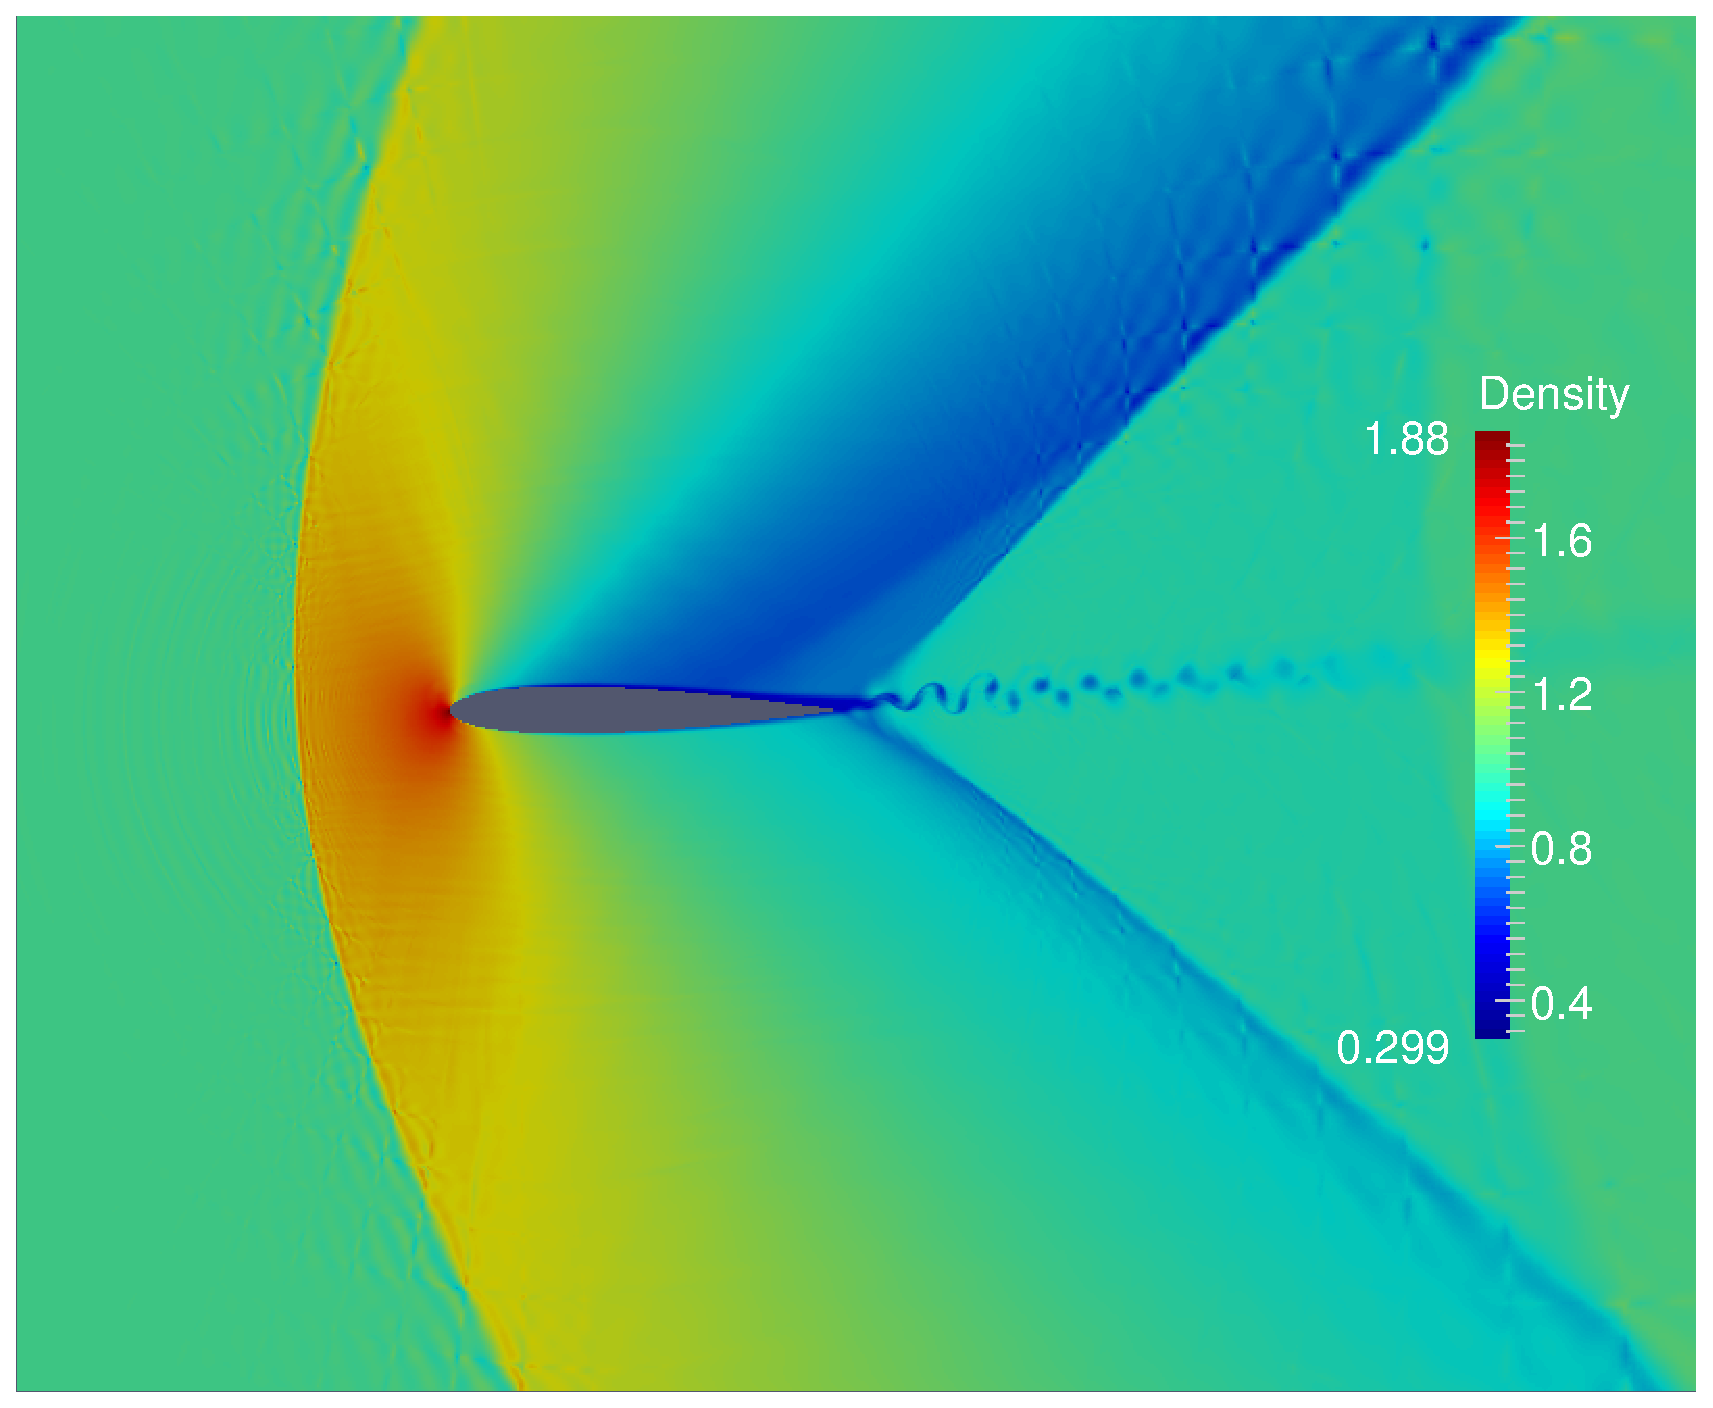
\includegraphics[width=.85\linewidth]{\aiaafigs /density-t1050010-jet.eps}
  \captionof{figure}{density contours for viscous flow at \gls{ma} = 1.2 over a NACA 0012 airfoil at 5$^{\circ}$ \gls{aoa} with polynomial order 6}
  \label{fig:visM1pt2-density}
\end{minipage}%
\begin{minipage}[t]{.5\textwidth}
  \centering
  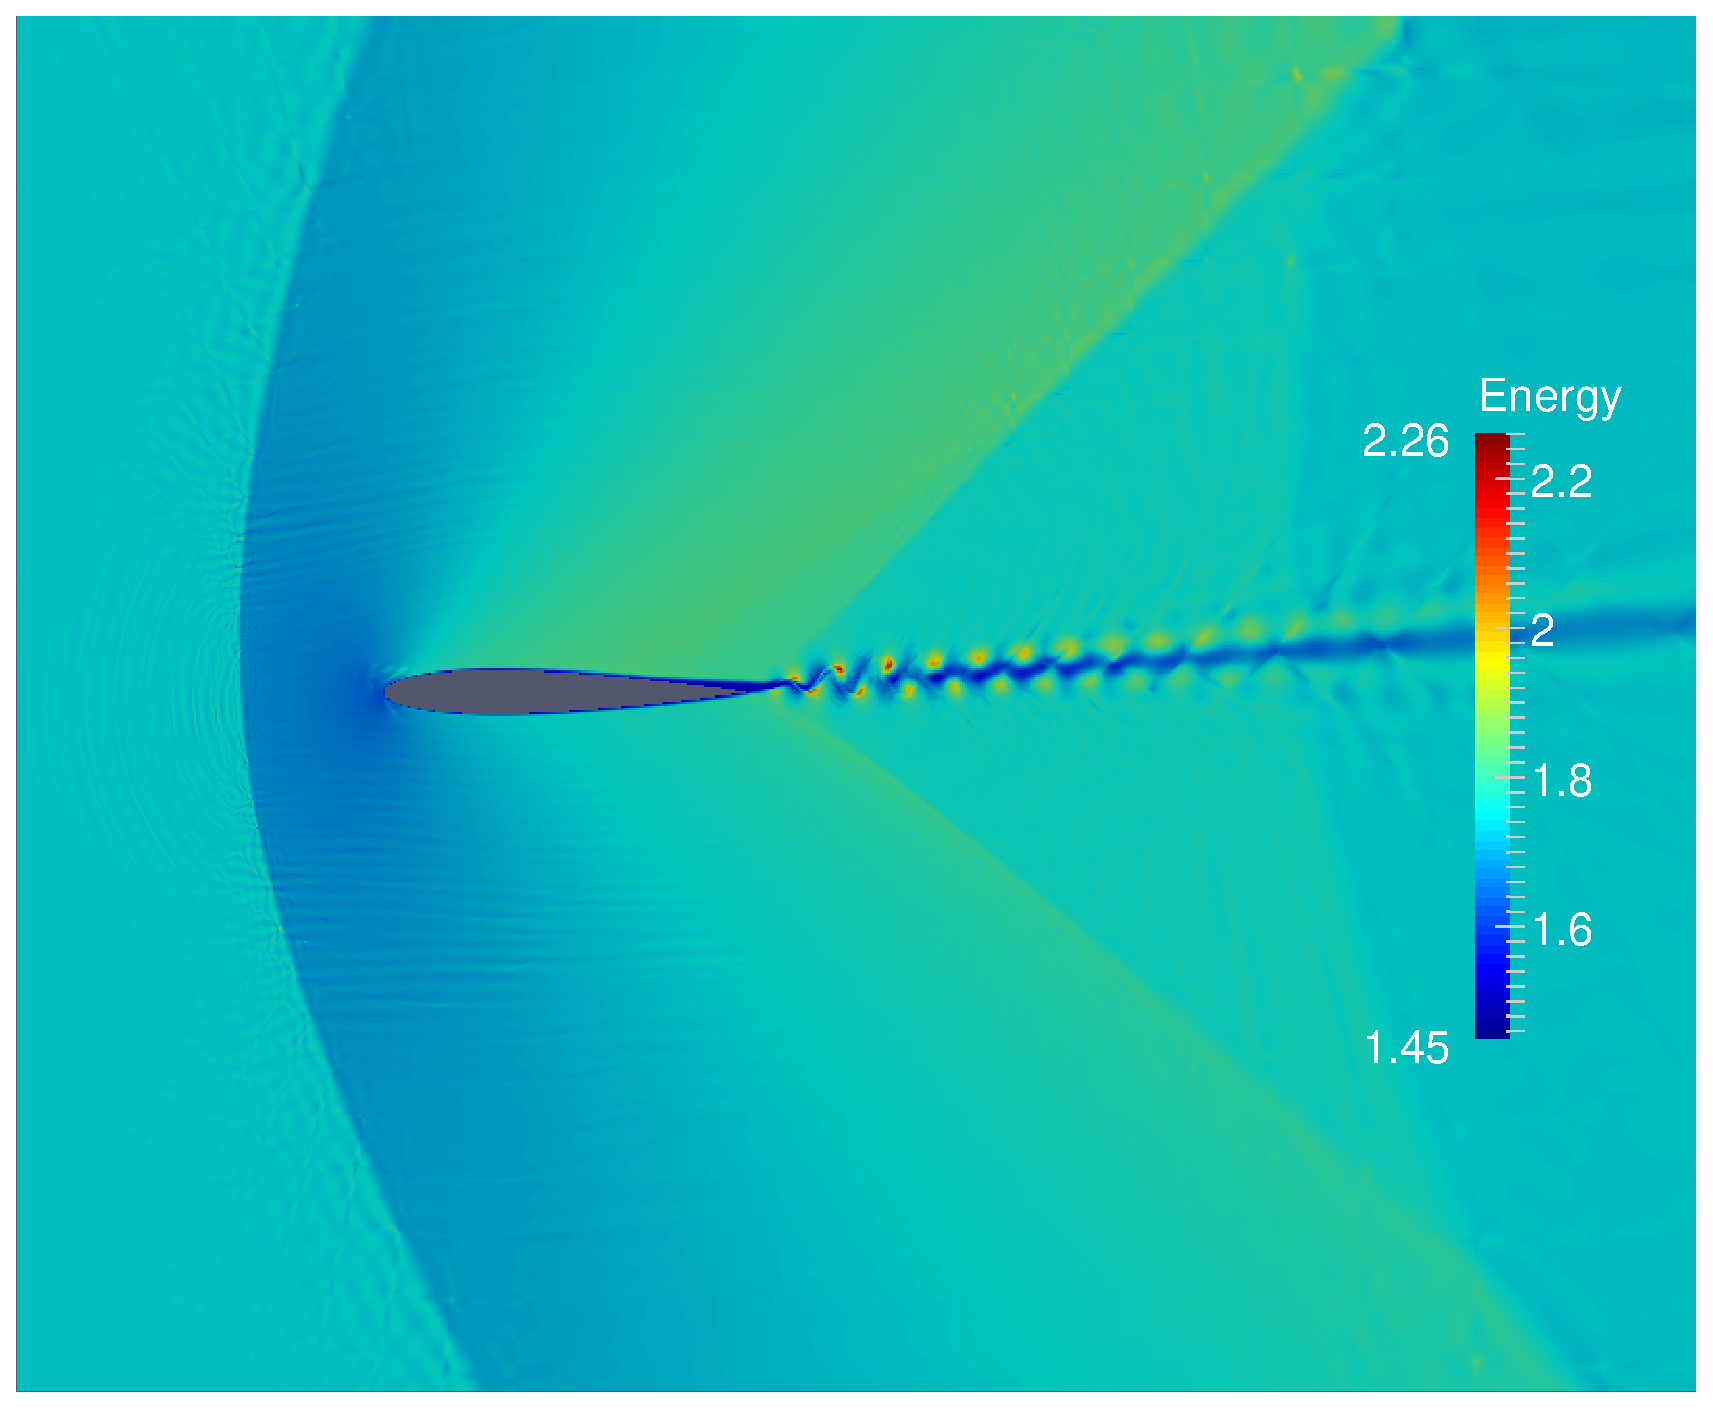
\includegraphics[width=.85\linewidth]{\aiaafigs /energy-t1050010-jet.eps}
  \captionof{figure}{Energy contours}
  \label{fig:visM1pt2-energy}
\end{minipage}
\end{figure} 

\begin{figure}[h] \tt
\centering
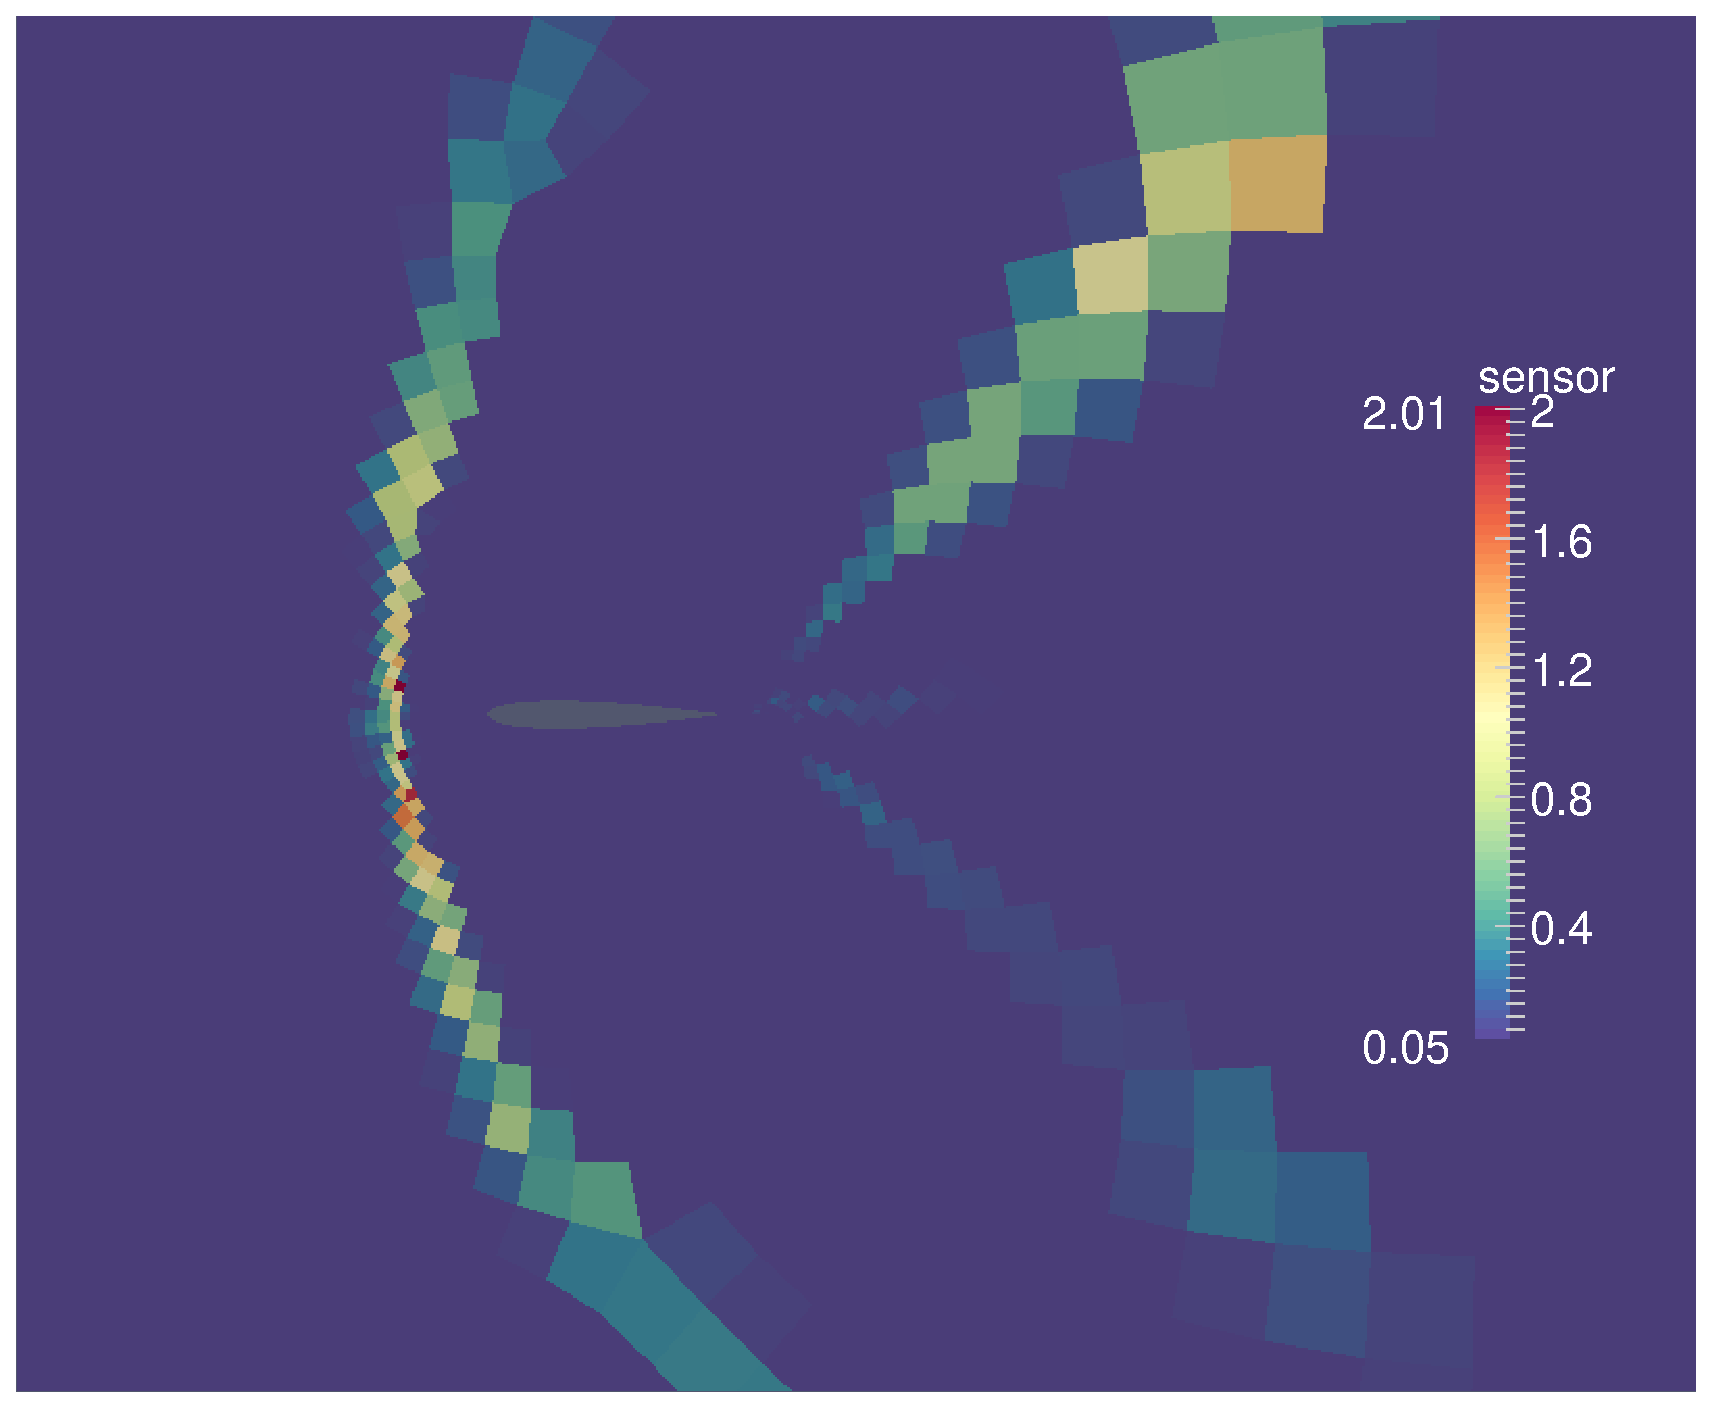
\includegraphics[width = 0.5\textwidth]{\aiaafigs /sensor-t1050010-spectral.eps}
\caption{Figure shows the elemental shock ``sensor'' for the \gls{ma} = 1.2 viscous case shown in figure ~\ref{fig:visM1pt2-density}. The shock sensor is just the maximum value of the enhanced kernel in each element}
\label{fig:sensor}
\end{figure}

\begin{figure}[h] \tt
\centering
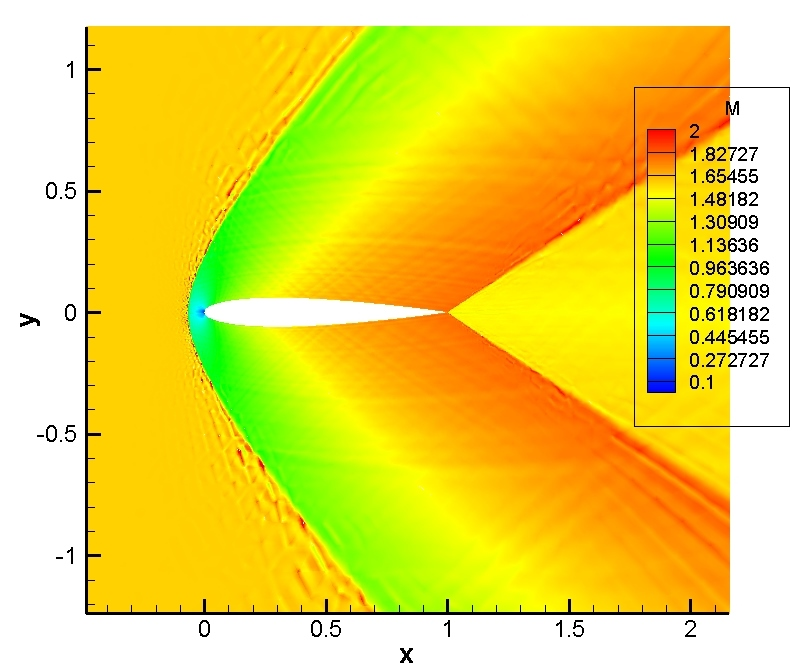
\includegraphics[width = 0.5\textwidth]{\aiaafigs /M1pt6order3-inv-720ktime-mach.jpg} \\
\caption{\gls{ma} contours for inviscid flow over NACA0012 at \gls{ma} = 1.6 and \gls{aoa} = $0^{\circ} $ on a triangle-mesh using Persson and Peraire's method and using artificial viscosity}
\label{fig:inv_mach}
\end{figure}

\begin{figure}
\centering
\begin{minipage}[t]{.55\textwidth}
  \centering
  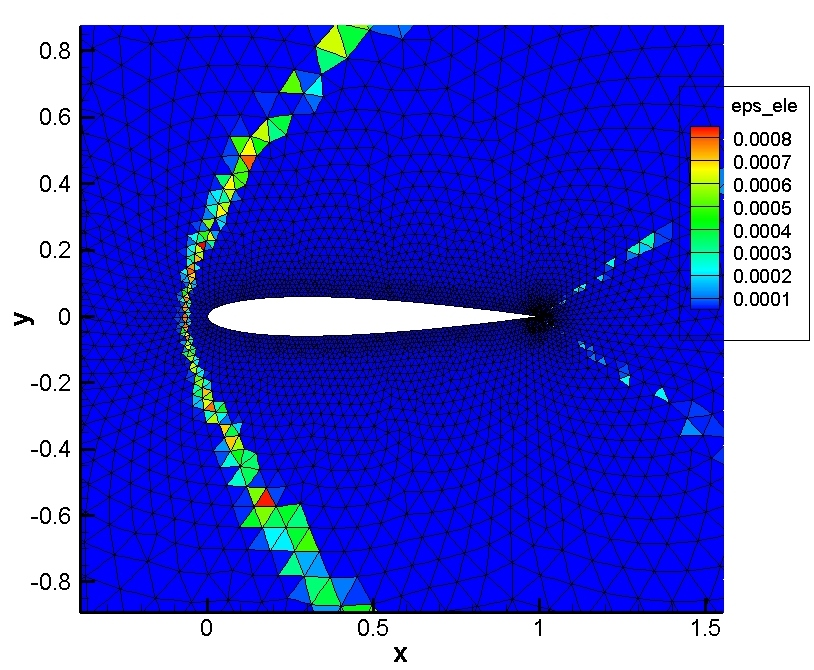
\includegraphics[width=.85\linewidth]{\aiaafigs /M1pt6-inv-av-ele-mesh}
  \caption{Element-wise \gls{av} coefficients for the inviscid \gls{ma}= 1.6 case}
  \label{fig:AV-ele}
\end{minipage}%
\begin{minipage}[t]{.55\textwidth}
  \centering
  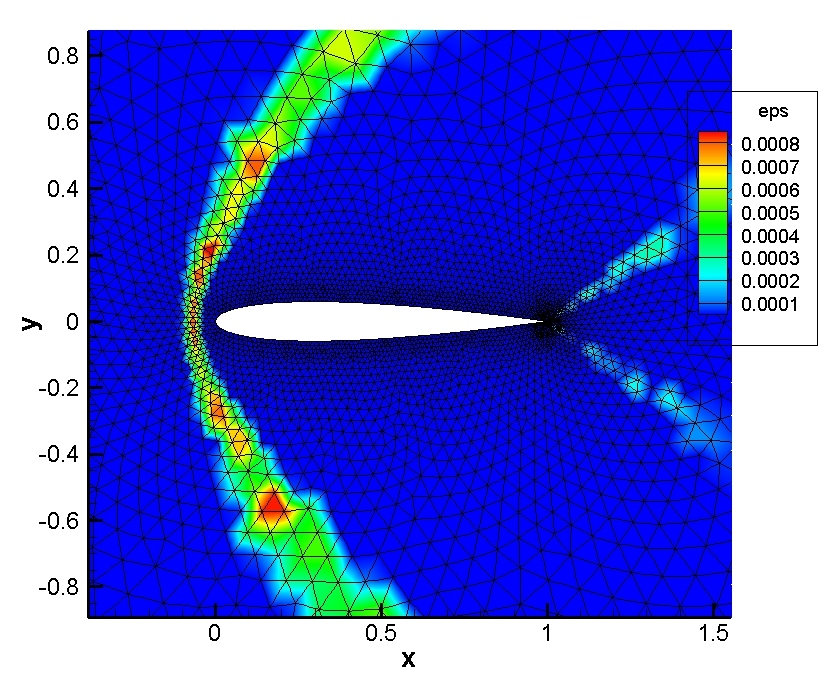
\includegraphics[width=.85\linewidth]{\aiaafigs /M1pt6-inv-av-mesh}
  \caption{\gls{av} coefficients with continuity enforcement}
  \label{fig:AV-cont}
\end{minipage}
\end{figure} 

\subsection{\gls{sa} Turbulence Model and Negative $\tilde\nu$ Modification}

The one equation \gls{sa} turbulence model is one of the more commonly used turbulence models used to solve attached and moderately separated aerodynamic flows~\cite{spalart1992one}. The added equation directly solves for turbulent eddy viscosity via advection, diffusion, production and dissipation. A modified form of the equation can be written as \cite{burgess2012robust,oliver2008high,moro2011navier}:
\begin{equation}
\begin{split}
	\frac{\partial}{\partial t}(\rho\tilde\nu) + \nabla\cdot(\rho\tilde\nu\boldsymbol{u}) = c_{b_1}\tilde S \rho\nu\psi &+ \frac{1}{\sigma}\left[\nabla\cdot((\mu + \mu\psi)\nabla\tilde\nu) + c_{b_2}\rho\nabla\tilde\nu\cdot\nabla\tilde\nu\right] \\&- c_{w_1}\rho f_w \left(\frac{\nu\psi}{d}\right)^2
\end{split}
\end{equation}

where $\tilde\nu$ is a modified version of the kinematic eddy viscosity and $\nu$ is the kinematic viscosity. The other variables are defined as:

\begin{align}
	 \mu_t =
	  \begin{cases}
	   \rho\tilde\nu f_{v_1} & \text{if } \tilde\nu \ge 0 \\
	   0       & \text{if } \tilde\nu < 0
	  \end{cases}
	  \quad \mbox{where} \quad f_{v_1} = \frac{\left(\frac{\rho\tilde\nu}{\mu}\right)^3}{\left(\frac{\rho\tilde\nu}{\mu}\right)^3 + c_{v_1}^3}
\end{align}

\begin{align}
	\tilde S &=
	\begin{cases}
	   S + \bar S & \text{if } \bar S \ge -c_{v_2}S \\
	   S + \frac{S(c_{v_2}^2 S + c_{v_3}\bar S)}{(c_{v_3} - 2c_{v_2})S - \bar S} & \text{if } \bar S \le -c_{v_2}S
	\end{cases}
\end{align}
\begin{align}
	S &= \sqrt{\boldsymbol{\omega}\cdot\boldsymbol{\omega}}
	\qquad \bar S = \frac{(\nu\psi)^2 f_{v_2}}{\kappa^2 d^2} \\
	f_{v_2} &= 1 - \frac{\psi}{1 + \psi f_{v_1}}
\end{align}

\begin{align}
	f_w &= g\left[\frac{1 + c_{w_3}^6}{g^6 + c_{w_3}^6}\right]^{1/6} 
	\qquad g = r + c_{w_2}(r^6 - r) 
	\qquad r = \frac{\nu\psi}{\tilde S \kappa^2 d^2}
\end{align}

where S is the magnitude of vorticity, d is the closest distance to a wall, $c_{b1} = 0.1355$, $\sigma = \frac{2}{3}$, $c_{b2} = 0.622$, $K = 0.41$, $\text{Pr}_t = 0.9$, $c_{v1} = 7.1$, $c_{v2} = 0.7$, $c_{v3} = 0.9$, $c_{w1} = \frac{c_{b1}}{K^2} + \frac{(1+c_{b2})}{\sigma}$, $c_{w2} = 0.3$, $c_{w3} = 2$.\\

The diffusion term, $\nabla\cdot(\rho\tilde\nu\boldsymbol{u})$, may become discontinuous in the first derivative leading to oscillations in high-order polynomials. This can lead to large negative values of the modified eddy viscosity term, $\tilde\nu$, significant enough to cause an unbounded solution. To prevent this, the following modification is introduced \cite{moro2011navier}.
\begin{align}
	\psi &=
	\begin{cases}
	   0.05log(1.0 + e^{(20.0\chi)}) & \text{if } \chi \le 10.0, \\
	   \chi & \text{if } \chi > 10.0,
	\end{cases} \\
	\chi &= \frac{\tilde\nu}{\nu}
\end{align}

\subsection{Large Eddy Simulation}\label{lesmodels}

In order to resolve all the scales of motion in a high \gls{re} number turbulent flow, the computational mesh would have to be exceedingly fine.
A practical solution is to employ the \gls{les} formulation, which only resolves the larger scales of motion and thus allows for the use of coarser meshes.

The effect of the unresolved or \gls{sgs} dynamics on the solution is accounted for by an \gls{sgs} model for the subgrid-scale stress $\tau_{ij}$, which is added to the viscous stress tensor $\sigma_{ij}$ given by (\ref{sigma}):

\begin{eqnarray}\label{tausgs}
\sigma_{ij} &&= 2 \mu S^d_{ij} + \tau_{ij},\\
S^d_{ij} &&= \frac 1 2 \l( \frac{\partial u_i}{\partial x_j} + \frac{\partial u_j}{\partial x_i} - \frac{2}{3} \delta_{ij}\frac{\partial u_k}{\partial x_k} \r).
\end{eqnarray}

The standard Smagorinsky model~\cite{smagorinsky1963} is available in \gls{hf}:
\begin{eqnarray}\label{smag}
\tau_{ij} &&= 2 \mu_t S^d_{ij}, \\
\mu_t &&= \rho C_S^2 \bigtriangleup^2 | S^d |,\\
| S^d | &&= \sqrt{2 S^d_{ij} S^d_{ij}},
\end{eqnarray}
where $\mu_t$ is the eddy viscosity, $C_S = 0.1$ is the Smagorinsky coefficient and $\bigtriangleup$ is the filter width. In \gls{hf} the filter width is given by (in 3D):
\begin{equation}
\bigtriangleup = \alpha (\text{vol})^{1/3},
\end{equation}
where $\alpha \geq 1$ is a user-defined scaling factor and vol is the element volume.

\gls{hf} also includes the \gls{wale} model~\cite{nicoud1999} and the Similarity model~\cite{bardina1980}.
The Similarity model incorporates a low-pass filtering operator, for which several choices are available in \gls{hf}: a discrete Gaussian filter\cite{lodato2012b}, a high-order commuting Vasilyev-type filter\cite{vasilyev1998,vasilyev2001} and a modal Vandermonde-type filter\cite{blackburn2003}.

The modal filter can be used on unstructured tetrahedral meshes. For details of these operators, see Lodato, Castonguay and Jameson~\cite{lodato2012b} and Bull and Jameson~\cite{bull2014a}. One can combine the similarity model with the Smagorinsky or \gls{wale} model to form a mixed \gls{sgs} model. The \gls{wsm} model, first proposed by Lodato et al.~\cite{lodato2009}, was used in simulations of the flow over a square cylinder (see Section~\ref{sqcyl}).

\subsection{Computing Architecture and Scalability}

The \gls{hf} code has been designed to work on multi-CPU as well as multi-CPU-\gls{gpu} platforms. The \gls{fr} method in its current form with explicit time-stepping has a great potential for parallelization. Since the solution points are not explicitly shared between elements, most of the computations are element-local enabling an efficient use of shared memory on \gls{gpu}s. Also, several computations are independent for each solution point and the highly parallelizable nature of \gls{gpu}s becomes very useful. A detailed description of the parallelization of the \gls{fr} method, along with scalability and performance analysis has been performed in~\cite{castonguay2011}.

% !TEX root = ../thesis.tex

\section{Verification and Validation}

\label{sec:verification}

% Manufactured solutions
% !TEX root = ../thesis.tex
\graphicspath{{figures_manufactured/}}% Set graphics path location


\subsection{Method of Manufactured Solutions}

This section describes the test of \gls{hf}'s spatial order of accuracy using the \gls{mms} in 2D and 3D for viscous flows. As shown by Salari et. al~\cite{salari2000code}, the \gls{mms} test rigorously assesses the correctness of implementation of a solver of \gls{pde}s. Simplex elements are crucial for simulations in unstructured meshes and have a more complex implementation than squares and hexahedra. As a result, we perform the \gls{mms} test in grids using simplex elements.

The \gls{mms} test for \gls{ns} solvers requires checking the solver's solution against an exact solution. Such exact solution can be chosen arbitrarily. The \gls{ns} equations can be satisfied with this arbitrary solution by including a time-dependent source term in the equations. Then, we solve

\begin{equation}
\frac{\partial U}{\partial t} +  \nabla \cdot {\bf F} = S
\end{equation}

For the following tests, we selected a smooth exact solution, so aliasing does not pollute the results. We picked

\begin{equation}\label{eq:NSwithSource}
\begin{split}
U_{2D} = \l(
\begin{tabular}{c}
$\sin{(k(x+y) - \omega t)} + a$\\
$\sin{(k(x+y) - \omega t)} + a$\\
$\sin{(k(x+y) - \omega t)} + a$\\
$(\sin{(k(x+y) - \omega t)} + a)^2$
\end{tabular}
\r) \\
U_{3D} = \l(
\begin{tabular}{c}
$\sin{(k(x+y+z) - \omega t)} + a$\\
$\sin{(k(x+y+z) - \omega t)} + a$\\
$\sin{(k(x+y+z) - \omega t)} + a$\\
$\sin{(k(x+y+z) - \omega t)} + a$\\
$(\sin{(k(x+y+z) - \omega t)} + a)^2$
\end{tabular}
\r)
\end{split}
\end{equation}

To find the value of $S$, we plug the values of our selected $U$ into the left-hand side of Equation~\eqref{eq:NSwithSource} and simplify. The resulting expression is $S$. 
We let \gls{pr}$=0.72, \gamma = 1.4, k = \pi, \omega = \pi, a = 3.0$ and $\mu = 0.001$.

The meshes used have dimensions $[-1,1] \times [-1,1]$ in 2D and $[-1,1] \times [-1,1] \times [-1,1]$ in 3D. Periodic boundary conditions were applied on the boundaries of the square and cube domains. Uniform square and cubic meshes were created and then each element was subdivided into triangles or tetrahedra. Two triangles were created from each square, and six tetrahedra were created from each cube. Consequently, in 2D a $N \times N$ mesh contains $2N^2$ triangles, and in 3D a $N \times N \times N$ mesh contains $6N^3$ tetrahedra. 


In 3D, the time step was $1$e$-4$ seconds and 10 seconds of flow were simulated. In 2D, the time step was $1$e$-6$ seconds and 1 second of flow was simulated. The time-stepping scheme used was the low-storage, $4^\text{th}$ order accurate \gls{rk45} method. 


% !TEX root = ../thesis.tex
\begin{table}[htbp]
\centering
\begin{tabular}{ c c c c c c c} 
  
 \specialcell{Polynomial\vspace{0.2cm}\\ Order} & Mesh: & 2x2x2 & 4x4x4 & 8x8x8 & 16x16x16 & \specialcell{Overall Order \vspace{0.2cm}\\ of Accuracy} \\ 
 \hline 
 \multirow{2}{*}{$p = 1$} & $L_2$ error & 5.76e-01 & 1.35e-01 & 3.22e-02 & 7.90e-03 &   \\ 
  
   & $\mathcal{O}(L_2)$ &   & 2.10 & 2.06 & 2.03 & 2.06 \\ 
 \hline 
 \multirow{2}{*}{$p = 2$} & $L_2$ error & 4.09e-01 & 5.52e-02 & 6.87e-03 & 8.53e-04 &   \\ 
  
   & $\mathcal{O}(L_2)$ &   & 2.89 & 3.01 & 3.01 & 2.97 \\ 
 \hline 
 \multirow{2}{*}{$p = 3$} & $L_2$ error & 9.77e-02 & 5.97e-03 & 3.78e-04 &   &   \\ 
  
   & $\mathcal{O}(L_2)$ &   & 4.03 & 3.98 &   & 4.01 \\ 
 \hline 
 \multirow{2}{*}{$p = 4$} & $L_2$ error & 1.12e-02 & 6.39e-04 & 2.07e-05 &   &   \\ 
  
   & $\mathcal{O}(L_2)$ &   & 4.13 & 4.95 &   & 4.54 \\ 
 \hline 
 \multirow{2}{*}{$p = 5$} & $L_2$ error & 1.53e-01 & 5.08e-03 & 6.92e-05 &   &   \\ 
  
   & $\mathcal{O}(L_2)$ &   & 4.91 & 6.20 &   & 5.55 \\ 
 \hline 
 \end{tabular}
\caption{Accuracy of \gls{hf} for NS equations with source term in tetrahedral meshes at $t = 10$. $L_2$ error is the $L_2$-norm of the error in the energy field: $\rho e$}
\label{table:tetsError1} 
 \end{table}

% !TEX root = ../thesis.tex
\begin{table}[htbp]
\centering
\begin{tabular}{ c c c c c c c} 
  
 \specialcell{Polynomial\vspace{0.2cm}\\ Order}  & Mesh: & 2x2x2 & 4x4x4 & 8x8x8 & 16x16x16 & \specialcell{Overall Order \vspace{0.2cm}\\ of Accuracy} \\ 
 \hline 
 \multirow{2}{*}{$p = 1$} & $L_2$ error & 1.98e+01 & 9.57e+00 & 4.55e+00 & 2.19e+00 &   \\ 
  
   & $\mathcal{O}(L_2)$ &   & 1.05 & 1.07 & 1.06 & 1.06 \\ 
 \hline 
 \multirow{2}{*}{$p = 2$} & $L_2$ error & 1.17e+01 & 2.98e+00 & 7.10e-01 & 1.71e-01 &   \\ 
  
   & $\mathcal{O}(L_2)$ &   & 1.97 & 2.07 & 2.06 & 2.03 \\ 
 \hline 
 \multirow{2}{*}{$p = 3$} & $L_2$ error & 3.17e+00 & 3.81e-01 & 4.73e-02 &   &   \\ 
  
   & $\mathcal{O}(L_2)$ &   & 3.06 & 3.01 &   & 3.03 \\ 
 \hline 
 \multirow{2}{*}{$p = 4$} & $L_2$ error & 5.21e-01 & 4.27e-02 & 2.69e-03 &   &   \\ 
  
   & $\mathcal{O}(L_2)$ &   & 3.61 & 3.99 &   & 3.80 \\ 
 \hline 
 \multirow{2}{*}{$p = 5$} & $L_2$ error & 3.20e+00 & 1.88e-01 & 4.79e-03 &   &   \\ 
  
   & $\mathcal{O}(L_2)$ &   & 4.09 & 5.29 &   & 4.69 \\ 
 \hline 
 \end{tabular}
\caption{Accuracy of \gls{hf} for NS equations with source term in tetrahedral meshes at $t = 10$. $L_2$ error is the $L_2$-norm of the error in the gradient of the energy field:$\frac{\partial}{\partial x_i} (\rho e)$}
\label{table:tetsError2} 
 \end{table}

% !TEX root = ../thesis.tex

\begin{table}[htbp]

%\centering
  \hspace{-1.1cm}
\begin{tabular}{ c c c c c c c c} 

 \specialcell{Polynomial\vspace{0.2cm}\\ Order}  & Mesh: & 4x4 & 8x8 & 16x16 & 32x32 & 64x64 & \specialcell{Overall Order \vspace{0.2cm}\\ of Accuracy}  \\ 
 \hline 
 \multirow{2}{*}{$p = 1$} & $L_2$ error & 7.92e-01 & 1.84e-01 & 4.36e-02 & 1.07e-02 & 2.68e-03 &   \\ 
  
   & $\mathcal{O}(L_2)$ &   & 2.10 & 2.08 & 2.03 & 2.00 & 2.05 \\ 
 \hline 
 \multirow{2}{*}{$p = 2$} & $L_2$ error & 1.29e-01 & 1.61e-02 & 1.95e-03 & 2.33e-04 & 2.86e-05 &   \\ 
  
   & $\mathcal{O}(L_2)$ &   & 3.00 & 3.05 & 3.06 & 3.03 & 3.04 \\ 
 \hline 
 \multirow{2}{*}{$p = 3$} & $L_2$ error & 1.01e-02 & 9.25e-04 & 5.71e-05 & 3.65e-06 & 2.35e-07 &   \\ 
  
   & $\mathcal{O}(L_2)$ &   & 3.45 & 4.02 & 3.97 & 3.96 & 3.88 \\ 
 \hline 
 \multirow{2}{*}{$p = 4$} & $L_2$ error & 2.60e-03 & 6.33e-05 & 2.00e-06 & 6.49e-08 & 3.62e-09 &   \\ 
  
   & $\mathcal{O}(L_2)$ &   & 5.36 & 4.98 & 4.95 & 4.16 & 4.88 \\ 
 \hline 
 \multirow{2}{*}{$p = 5$} & $L_2$ error & 7.15e-05 & 3.87e-06 & 6.31e-08 &   &   &   \\ 
  
   & $\mathcal{O}(L_2)$ &   & 4.21 & 5.94 &   &   & 5.07 \\ 
 \hline 
 \end{tabular}
\caption{Accuracy of \gls{hf} for NS equations with source term in triangular meshes at $t = 1$. $L_2$ error is the $L_2$-norm of the error in the energy field: $\rho e$}
\label{table:trisError1} 
 \end{table}

% !TEX root = ../thesis.tex
\hspace{-1.cm}
\begin{table}[htbp]
  \hspace{-1.2cm}
\begin{tabular}{ c c c c c c c c} 
  
 \specialcell{Polynomial\vspace{0.2cm}\\ Order} & Mesh: & 4x4 & 8x8 & 16x16 & 32x32 & 64x64 & \specialcell{Overall Order \vspace{0.2cm}\\ of Accuracy} \\ 
 \hline 
 \multirow{2}{*}{$p = 1$} & $L_2$ error & 1.61e+01 & 8.31e+00 & 3.81e+00 & 1.71e+00 & 7.84e-01 &   \\ 
  
   & $\mathcal{O}(L_2)$ &   & 0.96 & 1.12 & 1.15 & 1.13 & 1.10 \\ 
 \hline 
 \multirow{2}{*}{$p = 2$} & $L_2$ error & 4.05e+00 & 8.16e-01 & 1.90e-01 & 4.54e-02 & 1.11e-02 &   \\ 
  
   & $\mathcal{O}(L_2)$ &   & 2.31 & 2.11 & 2.06 & 2.04 & 2.12 \\ 
 \hline 
 \multirow{2}{*}{$p = 3$} & $L_2$ error & 4.71e-01 & 6.39e-02 & 7.03e-03 & 7.75e-04 & 8.84e-05 &   \\ 
  
   & $\mathcal{O}(L_2)$ &   & 2.88 & 3.18 & 3.18 & 3.13 & 3.11 \\ 
 \hline 
 \multirow{2}{*}{$p = 4$} & $L_2$ error & 1.01e-01 & 4.30e-03 & 2.31e-04 & 1.41e-05 & 5.27e-06 &   \\ 
  
   & $\mathcal{O}(L_2)$ &   & 4.56 & 4.22 & 4.04 & 1.42 & 3.67 \\ 
 \hline 
 \multirow{2}{*}{$p = 5$} & $L_2$ error & 5.04e-03 & 2.50e-04 & 7.80e-06 &   &   &   \\ 
  
   & $\mathcal{O}(L_2)$ &   & 4.33 & 5.00 &   &   & 4.67 \\ 
 \hline 
 \end{tabular}
\caption{Accuracy of \gls{hf} for NS equations with source term in triangular meshes at $t = 1$. $L_2$ error is the $L_2$-norm of the error in the gradient of the energy field:$\frac{\partial}{\partial x_i} (\rho e)$}
\label{table:trisError2} 
 \end{table}


Tables \eqref{table:trisError1} and \eqref{table:tetsError1} show the spatial order of accuracy achieved when calculating the energy fields $\rho e$ in 2D and 3D, respectively. Tables \eqref{table:trisError2} and \eqref{table:tetsError2} show the order of accuracy for the gradient of the energy field $\frac{\partial }{\partial x_i}(\rho e)$ in 2D and 3D, respectively. Because of the exact solutions that were picked, the exact values of the gradients of $\rho e$ in the $x,y,z$ directions are equal.

As expected\cite{hesthaven2007nodal}, the order of accuracy of the solution is $p+1$ and the order of accuracy of the gradient of the solution is $p$, where $p$ is the order of the polynomial used to approximate the solution fields. In the fifth order simulations, the relatively large time step introduces errors larger than the spatial discretization errors. Hence we observe sub-optimal orders of convergence in the coarsest meshes.

%\begin{figure}
%\centering
%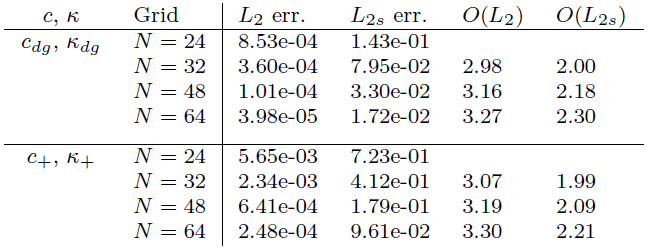
\includegraphics[height=35mm]{table_917} \\
%\caption{Accuracy of ESFR schemes for flow generated by a time-dependent source term on triangular grids, for the case of $p = 2$. The inviscid and viscous numerical fluxes were computed using a Rusanov flux with $\lambda = 1$ and a LDG flux with $\tau = 0.1$ and $\beta = \pm 0.5n$.}
%\label{fig:table_917}
%\end{figure}
%
%\begin{figure}
%\centering
%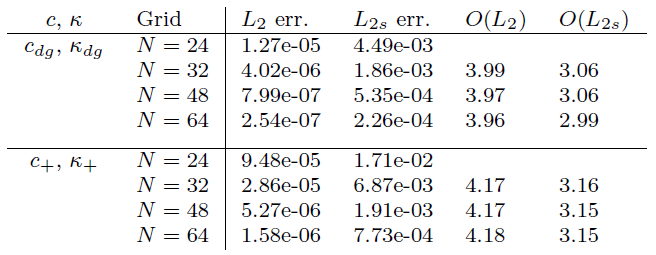
\includegraphics[height=35mm]{table_918} \\
%\caption{Accuracy of ESFR schemes for flow generated by a time-dependent source term on triangular grids, for the case of $p = 3$. The inviscid and viscous numerical fluxes were computed using a Rusanov flux with $\lambda = 1$ and a LDG flux with $\tau = 0.1$ and $\beta = \pm 0.5n$.}
%\label{fig:table_918}
%\end{figure}
%
%\begin{figure}
%\centering
%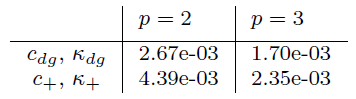
\includegraphics[height=20mm]{table_919} \\
%\caption{Explicit time-step limits ($\Delta t_{max}$) of ESFR schemes for flow generated by a time-dependent source term on the triangular grid with $\tilde{N} = 48$, for the cases of $p = 2$ and $3$. The inviscid and viscous numerical fluxes were computed using a Rusanov flux with $\lambda = 1$ and a LDG flux with $\tau = 0.1$ and $\beta = \pm 0.5n$.}
%\label{fig:table_919}
%\end{figure}
%
%\begin{figure}
%\centering
%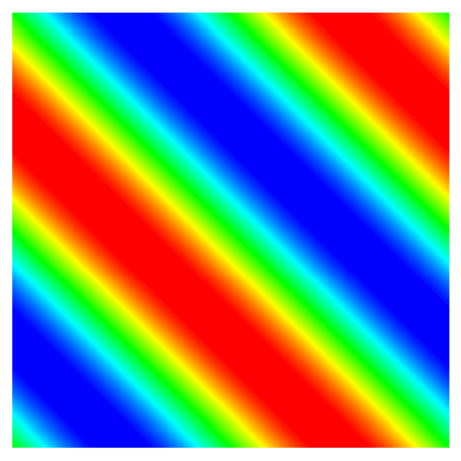
\includegraphics[height=60mm]{figure_912} \\
%\caption{Contours of energy obtained using the ESFR scheme with $c = c_+$ and $\kappa = \kappa_+$ on the triangular grid with $\tilde{N} = 32$ for the case of $p = 3$. The inviscid and viscous numerical fluxes were computed using a Rusanov flux with $\lambda = 1$ and a LDG flux with $\tau = 0.1$ and $\beta = \pm 0.5n$.}
%\label{fig:figure_912}
%\end{figure}
%
%\begin{figure}
%\centering
%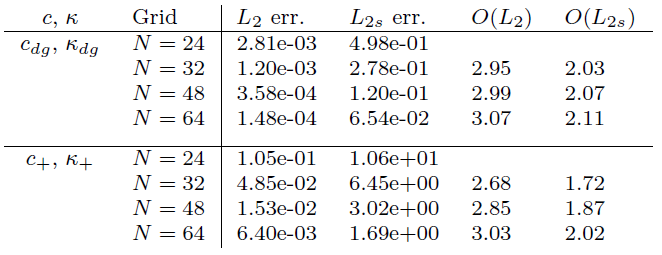
\includegraphics[height=35mm]{table_920} \\
%\caption{Accuracy of ESFR schemes for flow generated by a time-dependent source term on tetrahedral grids, for the case of $p = 2$. The inviscid and viscous numerical fluxes were computed using a Rusanov flux with $\lambda = 1$ and a LDG flux with $\tau = 0.1$ and $\beta = \pm 0.5n$.}
%\label{fig:table_920}
%\end{figure}
%
%\begin{figure}
%\centering
%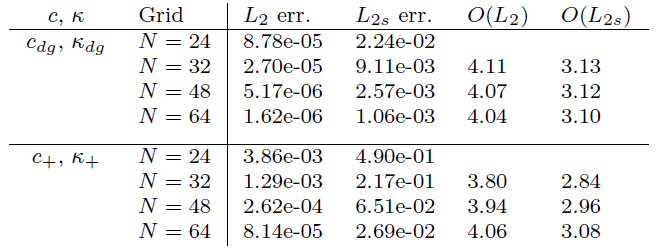
\includegraphics[height=30mm]{table_921} \\
%\caption{Accuracy of ESFR schemes for flow generated by a time-dependent source term on tetrahedral grids, for the case of $p = 3$. The inviscid and viscous numerical fluxes were computed using a Rusanov flux with $\lambda = 1$ and a LDG flux with $\tau = 0.1$ and $\beta = \pm 0.5n$.}
%\label{fig:table_921}
%\end{figure}
%
%\begin{figure}
%\centering
%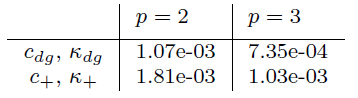
\includegraphics[height=15mm]{table_922} \\
%\caption{Explicit time-step limits ($\Delta t_{max}$) of ESFR schemes for flow generated by a time-dependent source term on the triangular grid with $\tilde{N} = 48$, for the cases of $p = 2 and 3$. The inviscid and viscous numerical fluxes were computed using a Rusanov flux with $\lambda = 1$ and a LDG flux with $\tau = 0.1$ and $\beta = \pm 0.5n$.}
%\label{fig:table_922}
%\end{figure}
%
%\newpage
%\begin{figure}
%\centering
%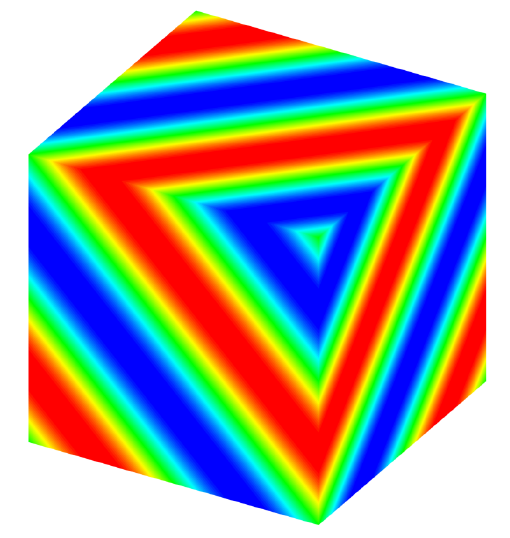
\includegraphics[height=60mm]{figure_913} \\
%\caption{Contours of energy obtained using the ESFR scheme with $c = c_+$ and $\kappa = \kappa_+$ on the tetrahedral grid with $\tilde{N} = 32$ for the case of $p = 3$. The inviscid and viscous numerical fluxes were computed using a Rusanov flux with $\lambda = 1$ and a LDG flux with $\tau = 0.1$ and $\beta = \pm 0.5n$.}
%\label{fig:figure_913}
%\end{figure}


% Flat plate
% !TEX root = ../thesis.tex
\graphicspath{{\aiaadir /figures_flatplate/}}% Set graphics path location

\subsection{Subsonic laminar flat-plate}

Computations of the flow over a subsonic flat-plate have been performed and validated against the Blasius' solution for laminar boundary layer. The flow conditions are \gls{ma} $0.5$, 0$\degr$ angle of attack and \gls{re} $1\cdot10^6$ based on the plate length. The governing equations are the 2D \gls{ns} equations with constant ratio of specific heats of $1.4$, Prandtl number of $0.72$ and constant dynamic viscosity of $1.827\cdot 10^{-5} Pa \cdot s$.

\begin{center} 
    \begin{tabular}{l*{7}{c}r}
    Mesh & First cell height & \specialcell{\# of cells in \vspace{0.2cm}\\boundary layer} & $p_3$ & $p_4$ & $p_5$ & $p_6$ \\ \hline
    Mesh a0 (140 = 14x10) & 0.00075 & 2 & $\times$ & $\times$ & $\times$ & \Checkmark \\ \hline
    Mesh a1 (560 = 28x20) & 0.000375 & 4 &  $\times$ & $\times$ & \Checkmark & \Checkmark \\ \hline
    Mesh a2 (2240 = 56x40) & 0.0001875 & 8 & $\times$ & \Checkmark & \Checkmark & \Checkmark \\ \hline
    Mesh a3 (8960 = 112x80) & 0.0000935 & 16 & \Checkmark & \Checkmark & \Checkmark & \Checkmark \\
    \hline
    \end{tabular} 
      \captionof{table}{\gls{hf} convergence using different grids and polynomial order. $\times$ / \Checkmark indicates not converged/converged resp.} \label{tab:convergence} 
\end{center}

The objective of this study is to determine the minimum number of elements and the order of polynomial required to converge the flat-plate simulation using \gls{hf}. Four different numerical grids have been used in this study (2, 4, 8, 16 elements inside the boundary layer) and four polynomial orders ($p_3$--$p_6$). The results, summarized in Table \ref{tab:convergence}, show that a minimum number of elements is needed in the boundary layer depending on the polynomial order to obtain satisfactory convergence (free from inter-element jumps).

\begin{figure}
\begin{center}
\begin{minipage}[t]{0.48\columnwidth}
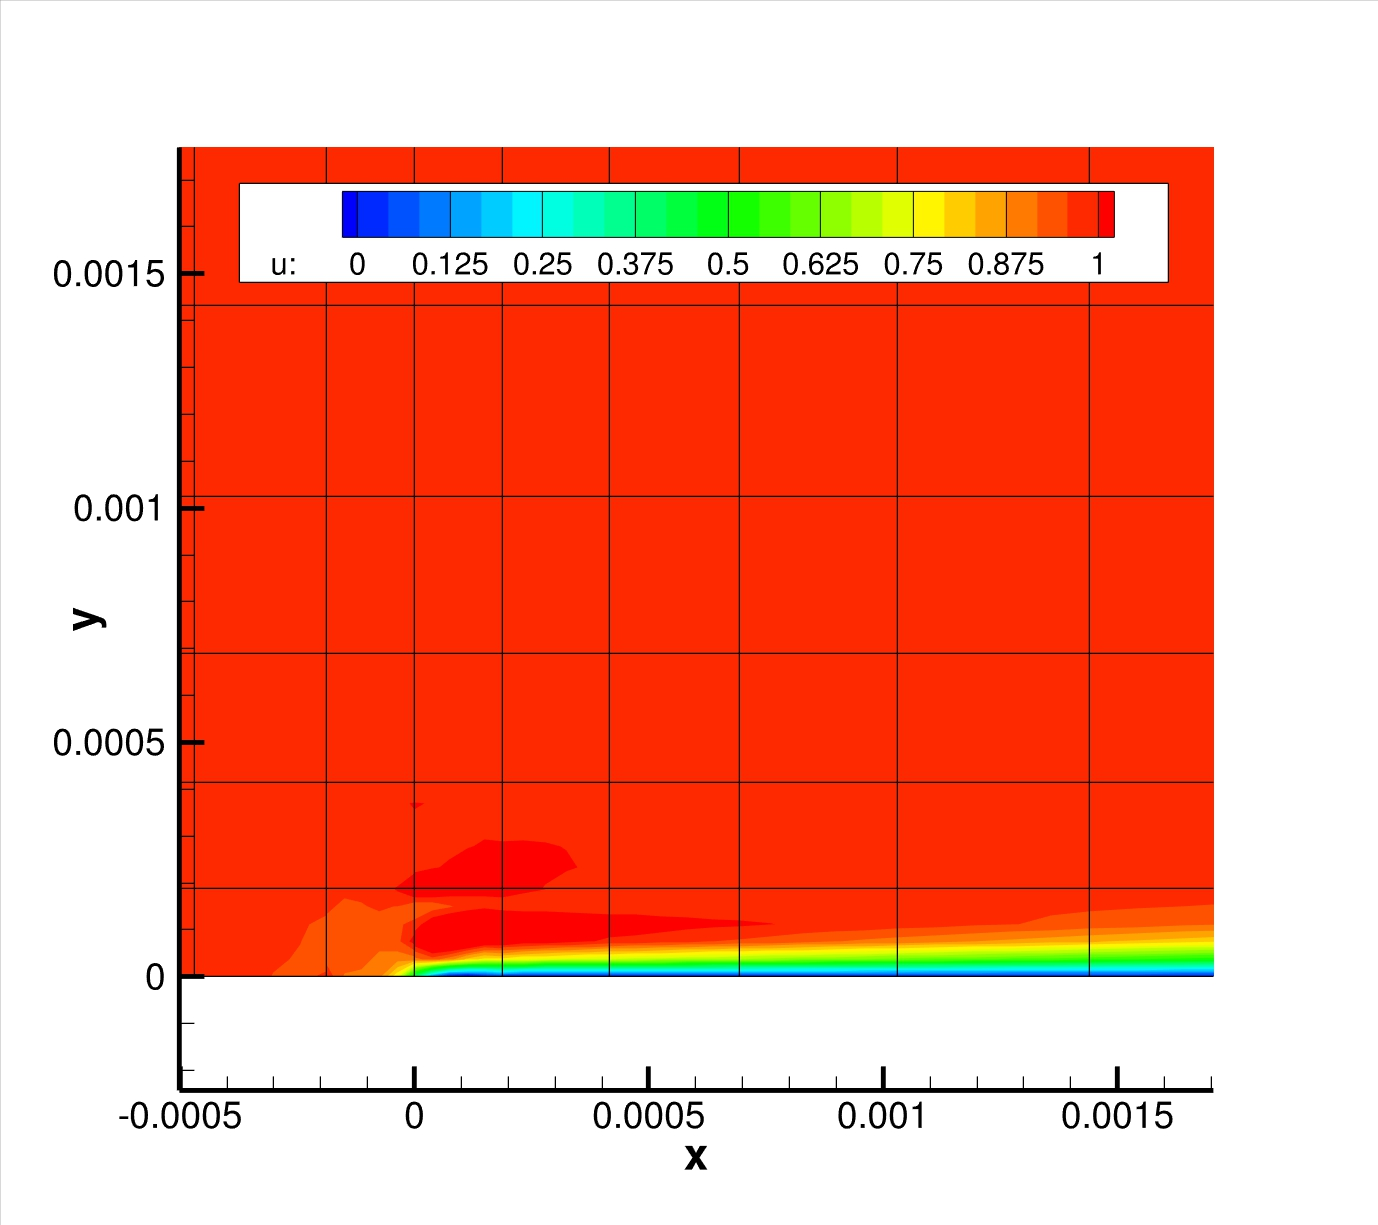
\includegraphics[width = \textwidth,clip=]{LeadingEdge.jpg}
\caption{Detail of the flat-plate leading edge (x=0.0, mesh a2).}
\label{fig:LeagingEdge}
\end{minipage}
\hfill
\begin{minipage}[t]{0.48\columnwidth}
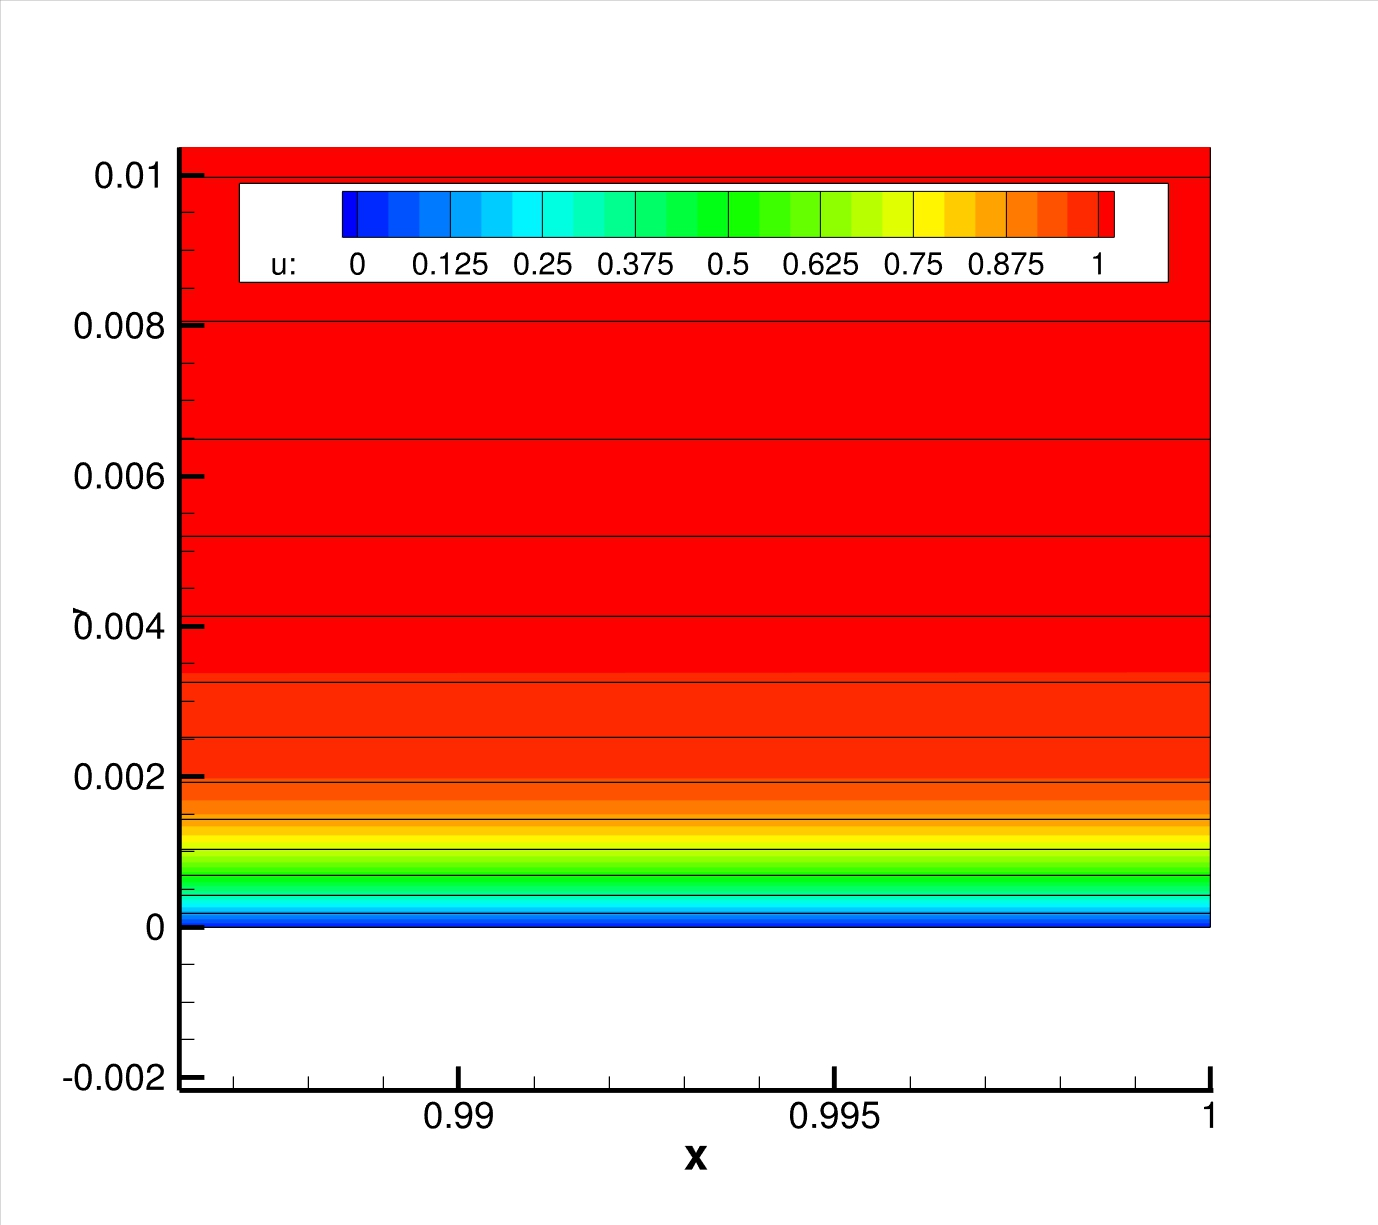
\includegraphics[width = \textwidth,clip=] {EndPlate.jpg}
\caption{Flow solution at the end of the flat-plate (x=1.0, mesh a2).}
\label{fig:TrailingEdge}
\end{minipage}
\end{center}
\end{figure}

The results are compared with the Blasius' solution for laminar boundary layer with satisfactory results, and some details of the solutions are presented in Fig. \ref{fig:LeagingEdge} (leading edge), and Fig. \ref{fig:TrailingEdge} (end of the flat-plate). It is important to note that in this particular case (mesh a2) the flat-plate boundary layer is captured using 8 elements, while in a second order solver it would be necessary of the order of ~30 elements inside the boundary layer.

\begin{figure}
\begin{center}
\begin{minipage}[t]{0.48\columnwidth}
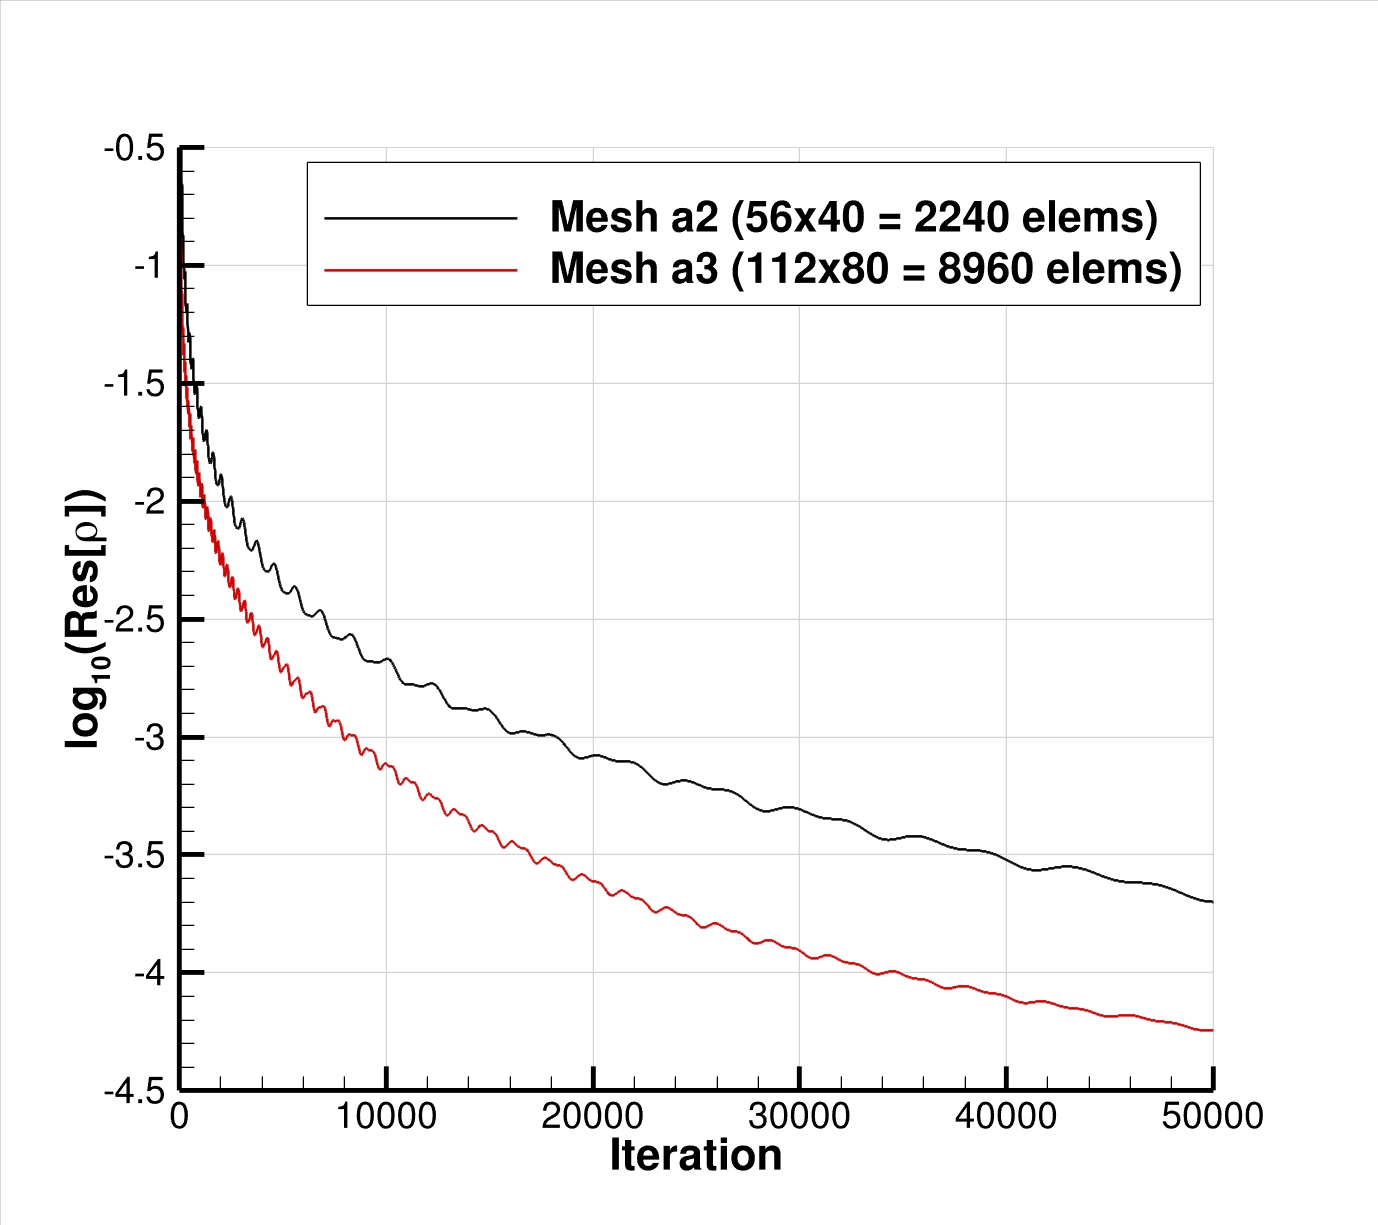
\includegraphics[width = \textwidth]{CompMesh.jpg}
\caption{Convergence comparison (3$^{rd}$ order, finest grids).}
\label{fig:ComparisonOrder}
\end{minipage}
\hfill
\begin{minipage}[t]{0.48\columnwidth}
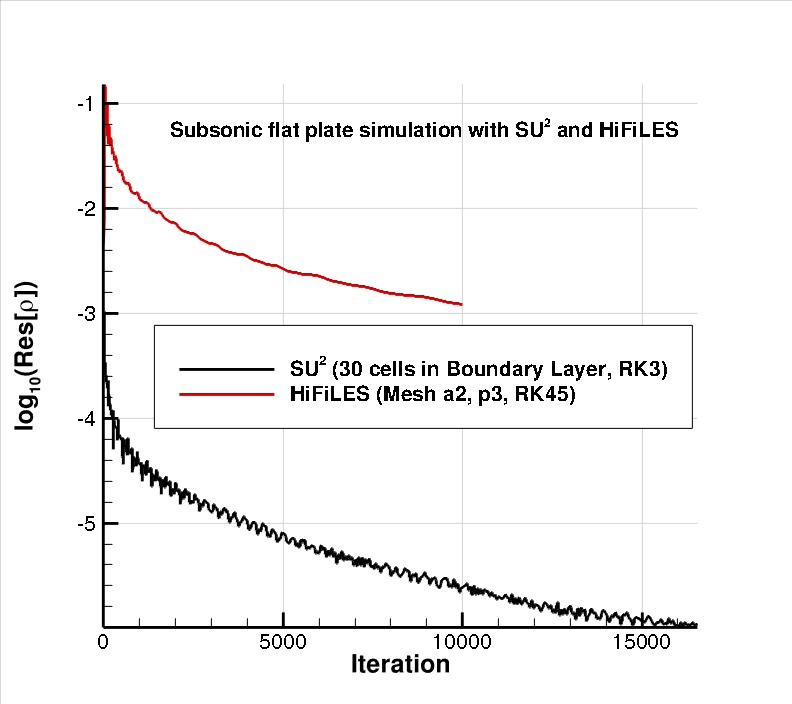
\includegraphics[width = \textwidth] {CompSu2.jpg}
\caption{Comparison of \gls{hf} with SU2 using a similar time integration scheme.}
\label{fig:Comparison_SecondOrder}
\end{minipage}
\end{center}
\end{figure}

To finalize, it is critical to note that the absence of a local time stepping technique in \gls{hf} increases the required number of iterations to obtain a converged solution. However, we have noticed an improvement of the rate of convergence as we refine the grid (see Fig. \ref{fig:ComparisonOrder}). The obtained convergence rate is comparable to a second order numerical code (e.g. SU2~\cite{palacios2013stanford,palacios14}) running using a similar numerical time integration (see Fig.~\ref{fig:Comparison_SecondOrder}).


% Circular cylinder
% !TEX root = ../thesis.tex
\graphicspath{{\aiaadir /figures_cylinder/}}% Set graphics path location

\subsection{Circular Cylinder}

The classic test case of laminar flow past a circular cylinder at low \gls{re} number has also been chosen as a verification and validation case for the 2D \gls{ns} equations in \gls{hf}, and the results are compared to existing experimental data and simulation results~\cite{park1998}. Two separate cases are computed: first, the steady flow past the cylinder at \gls{re}$= 20$, and second, the unsteady flow past the cylinder at \gls{re}$= 100$, where \gls{re} is based upon the diameter of the cylinder. For both cases, \gls{ma} number is set to 0.1 in order to recover nearly incompressible flow for comparisons with the existing incompressible results. The remaining flow conditions are $0\degr$ angle of attack, a constant ratio of specific heats of $1.4$, a Prandtl number of $0.72$, a free-stream temperature of $300K$, and a free-stream dynamic viscosity of $1.853\cdot 10^{-5} Pa \cdot s$ (laminar viscosity varies according to Sutherland's law during the simulation).

The two simulations are performed with third order polynomials on a mesh with $4988$ total elements that contains quadrilateral elements near the body of the cylinder and triangular elements out to the far-field. There is a small refinement box immediately downstream of the cylinder to help resolve features in the wake. The rectangular far-field boundaries are located approximately 30 diameters away from the cylinder in the upstream, upward, and downward directions and 50 diameters away in the downstream direction. A view of the mesh near the cylinder surface is show in Fig.~\ref{cylinder_1}.

\begin{figure}

    \subfloat[Zoom view of the mesh near the cylinder.]{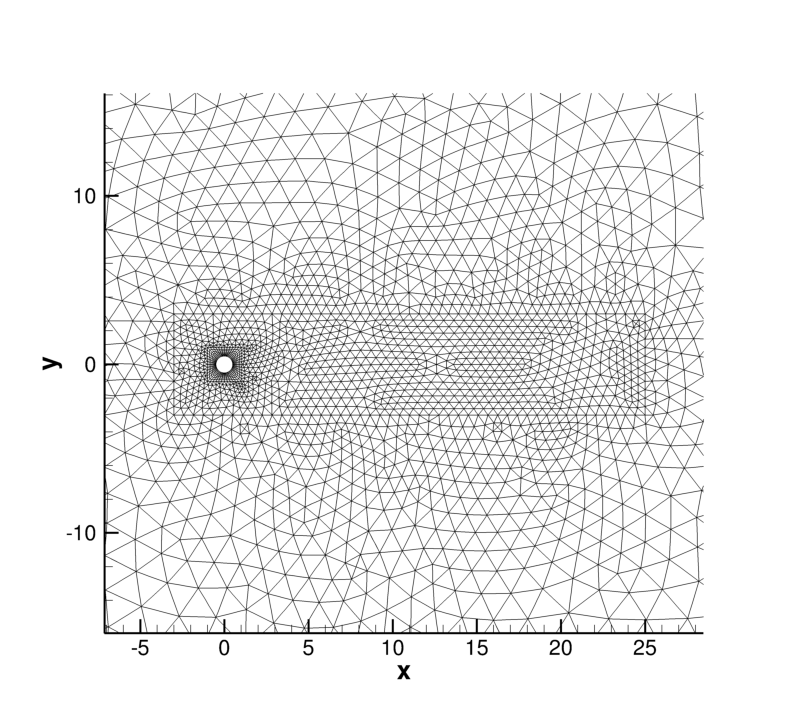
\includegraphics[width = 0.5\textwidth]{cylinder_mesh.png}}
    \subfloat[X-velocity contours and streamlines around the circular cylinder for $Re = 20$.]{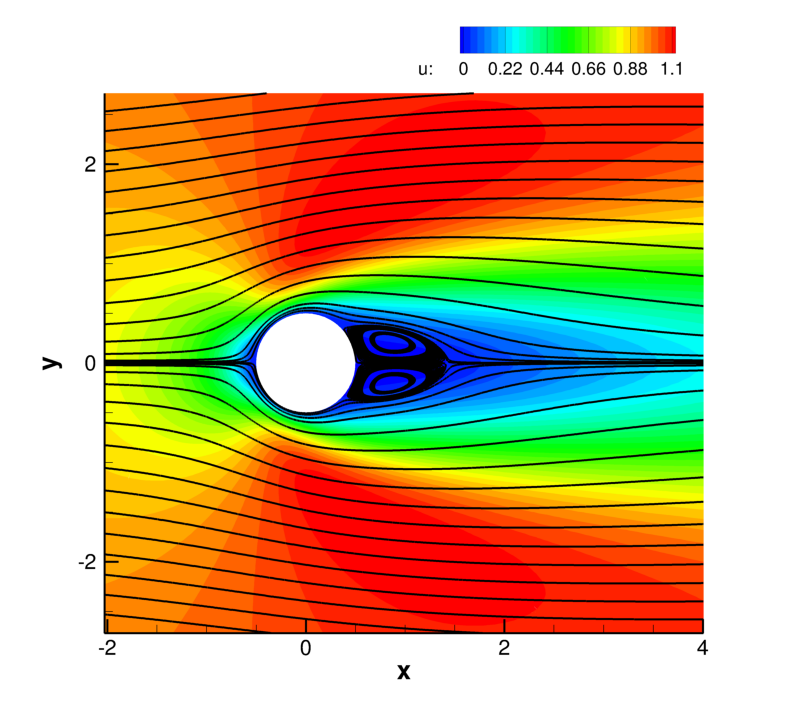
\includegraphics[width = 0.5\textwidth]{cylinder_streamlines.png}}
    
  \caption{The mesh for the circular cylinder simulations along with x-velocity contours for the $Re = 20$ case.}
  \label{cylinder_1}
\end{figure}

The flow around the cylinder for \gls{re}$= 20$ is steady, and it features a large recirculation region behind the cylinder. Fig.~\ref{cylinder_1} presents x-velocity contours around the cylinder along with streamlines. The length of the recirculation region can be determined from the streamlines, and a length of approximately one cylinder diameter agrees well with reported results for \gls{re}$= 20$. The coefficient of drag computed by \gls{hf} is $2.043$, which is close to the value of $2.01$ reported by Park et al.~\cite{park1998} Pressure contours around the cylinder are shown in Fig.~\ref{cylinder_2}.

\begin{figure}

    \subfloat[Pressure contours for the $Re = 20$ case.]{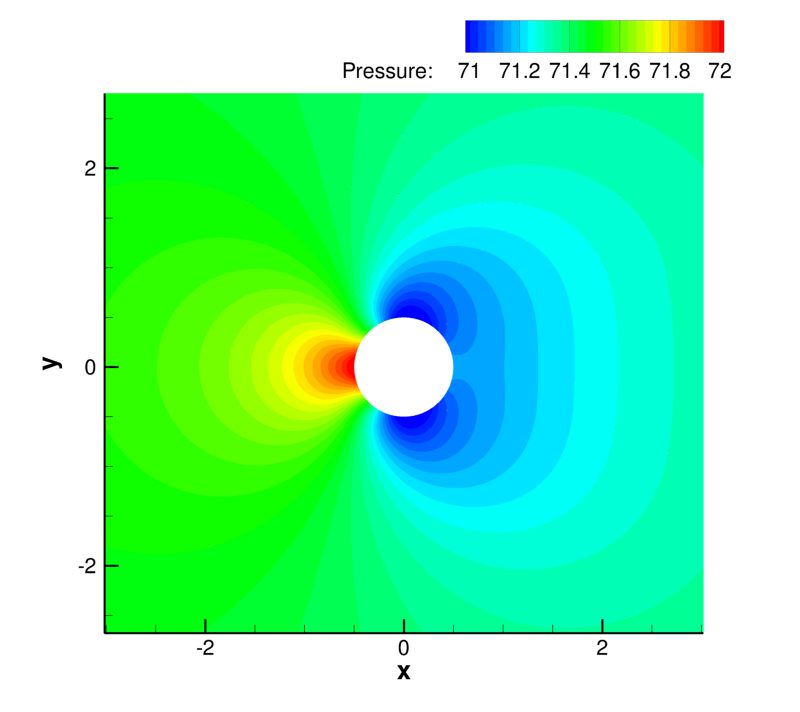
\includegraphics[width = 0.5\textwidth]{cylinder_pressure_re20.png}}
    \subfloat[Pressure contours for the $Re = 100$ case.]{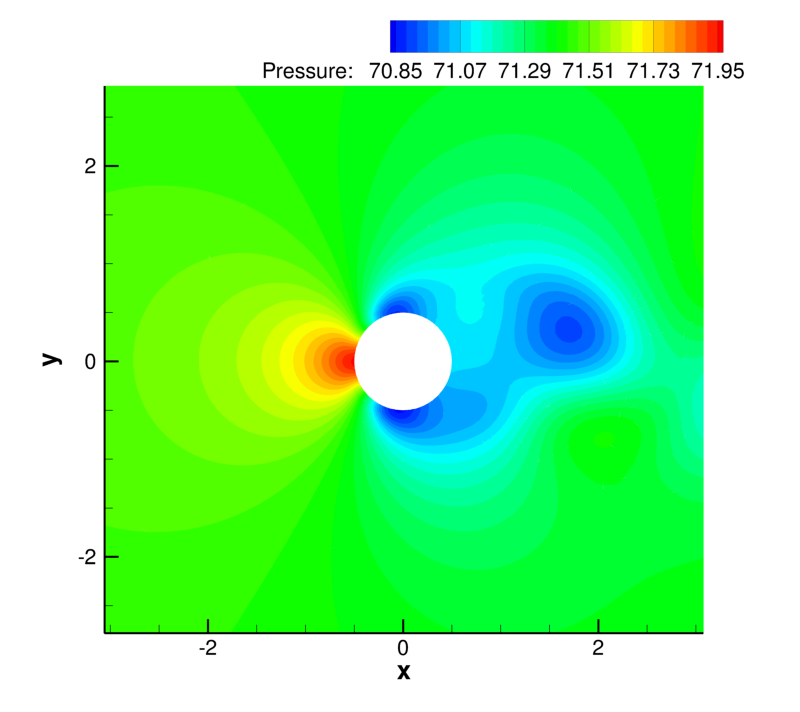
\includegraphics[width = 0.5\textwidth]{cylinder_pressure_re100.png}}

  \caption{Pressure contours for the steady and unsteady (instantaneous) cylinder cases.}
  \label{cylinder_2}
\end{figure}

When \gls{re} is increased to $100$, the flow around the cylinder becomes unsteady and exhibits periodic vortex shedding. This periodic shedding in the wake behind the cylinder can be seen in the instantaneous contours of x-velocity and vorticity in Fig.~\ref{cylinder_3}, and it also results in periodic fluctuations in the force coefficients on the cylinder. \gls{hf} reports an average drag coefficient of $1.339$ with a maximum deviation from this value of $0.0092$, which agree excellently with the values reported by Park et al.~\cite{park1998} of $1.33$ and $0.0091$ for the average $C_d$ and maximum deviation from it, respectively.  Instantaneous pressure contours for the \gls{re}$= 100$ case can be seen in Fig.~\ref{cylinder_2}. The asymmetry that is visible in the pressure contours contributes to the variability in the drag coefficient.

\begin{figure}
    \subfloat[X-velocity contours around the circular cylinder for \gls{re}$= 100$.]{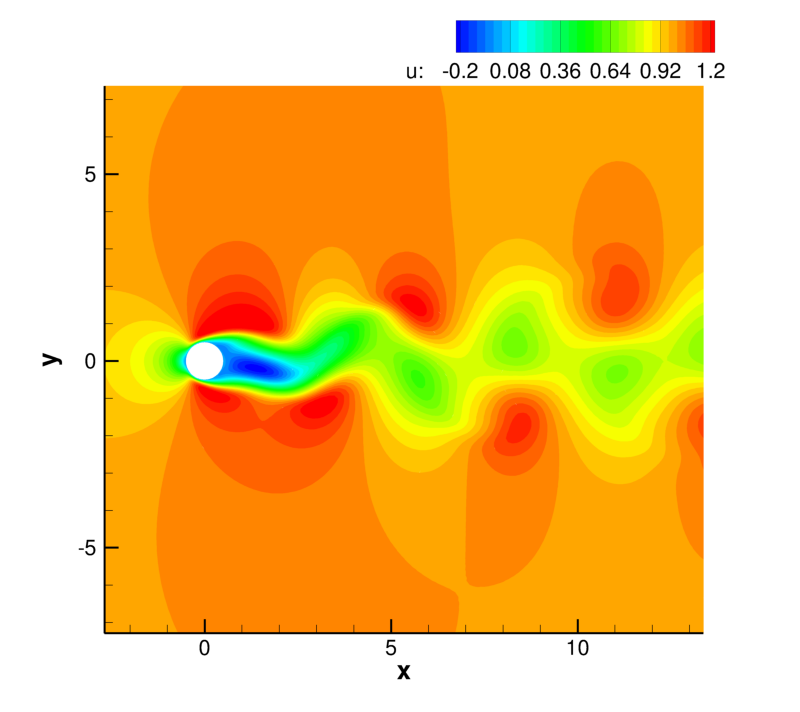
\includegraphics[width = 0.5\textwidth]{cylinder_xvelocity_re100.png}}
    \subfloat[Vorticity contours for the \gls{re}$= 100$ case.]{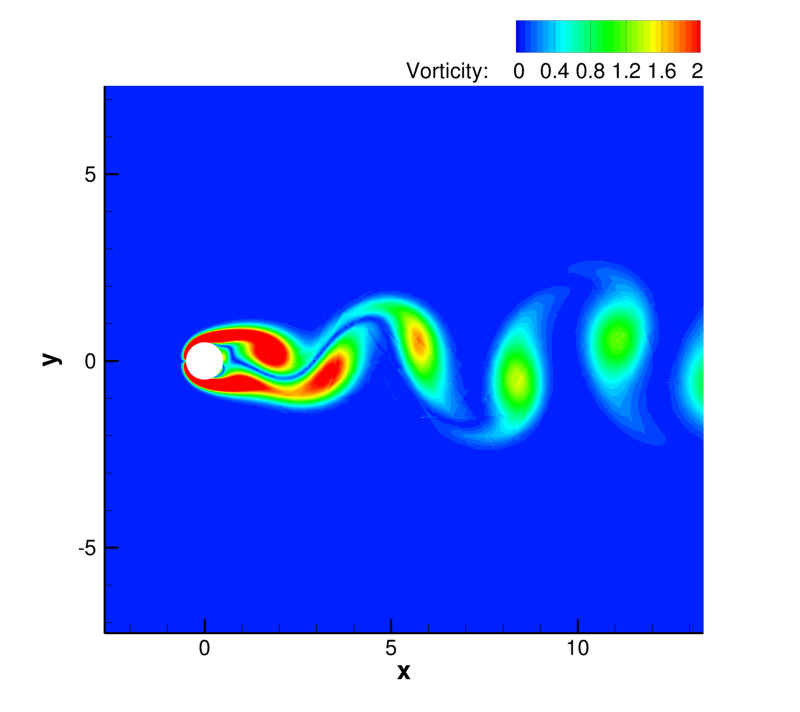
\includegraphics[width = 0.5\textwidth]{cylinder_vorticity_re100.png}}

  \caption{Instantaneous solution contours for the unsteady cylinder case.}
  \label{cylinder_3}
\end{figure}

% SD7003 section
% !TEX root = ../thesis.tex
\graphicspath{{\aiaadir /figures_SD7003/}}% Set graphics path location

\subsection{SD7003 airfoil at 4$\degr$ angle of attack}\label{sd7003airfoil}

Abundant literature documents flow around a SD7003 infinite wing and airfoil. Hence, physical experiments \cite{ol2005comparison,radespiel2007numerical} and numerical simulations \cite{galbraith2008implicit,visbal2009high,castonguay2010simulation,persson2011high,uranga2011implicit} of flow over this geometry can be used to benchmark \gls{hf}.

The simulations on the 2D geometry were performed on a circular domain with a radius of $50c$, where $c$ is the airfoil's cord length, centered at the leading edge of the airfoil. The boundary conditions are characteristic on the outer edge and adiabatic no-slip wall on the airfoil. The Mach number for all simulations was \gls{ma}$= 0.2$. The reported lift and drag coefficients in Table \eqref{table:sdAirfoilForce} correspond to the average of lift and drag coefficients over $13$ periods after the flow reached a pseudo-periodic state. More details are provided by Williams~\cite{williams2013thesis}. 

\begin{table}[htbp]
\centering
\begin{tabular}{ l| l l| l l| l l} 
  
 &  \multicolumn{2}{|c|}{$Re = 10K$}  & \multicolumn{2}{|c|}{$Re = 22K$} & \multicolumn{2}{|c}{$Re = 22K$}  \\ 
 Source & $C_L$ & $C_D$ & $C_L$ & $C_D$ & $C_L$ & $C_D$   \\ 
\hline
 Uranga et al.\cite{uranga2011implicit} & 0.3755 & 0.04978 & 0.6707 & 0.04510 & 0.5730 & 0.02097  \\ 
$c_{dg},\kappa_{dg}$ & 0.3719 & 0.04940 & 0.6722 & 0.04295 & 0.5831 & 0.01975 \\ 
$c_{+},\kappa_{+}$ & 0.3713 & 0.04935 & 0.6655 & 0.04275 & 0.5774 & 0.02005  \\ 
 \end{tabular}
\caption{Time-averaged values of the lift and drag coefficients for the SD7003 airfoil flows with $Re = 10,000, 22,000, 60,000$}
\label{table:sdAirfoilForce} 
 \end{table}

\begin{figure}[htbp]
\centering
\subfloat[Density contours]{
\includegraphics*[trim=0 0 0 0,width=0.48\textwidth]{figure_935a}}
\subfloat[Vorticity contours]{
\includegraphics*[trim=0 0 0 0,width=0.48\textwidth]{figure_935b}}\\

\caption{Density and vorticity contours for the flow with \gls{re}$= 10,000$ around the SD7003 airfoil. $p=2$ on unstructured triangular grid with $N = 25,810$ elements}
\label{sdairfoilre10k}
\end{figure}

\begin{figure}[htbp]
\centering
\subfloat[Density contours]{
\includegraphics*[trim=0 0 0 0,width=0.48\textwidth]{figure_936a}}
\subfloat[Vorticity contours]{
\includegraphics*[trim=0 0 0 0,width=0.48\textwidth]{figure_936b}}\\

\caption{Density and vorticity contours for the flow with \gls{re}$= 22,000$ around the SD7003 airfoil. $p=2$ on unstructured triangular grid with $N = 25,810$ elements}
\label{sdairfoilre22k}
\end{figure}

\begin{figure}[htbp]
\centering
\subfloat[Density contours]{
\includegraphics*[trim=0 0 0 0,width=0.48\textwidth]{figure_937a}}
\subfloat[Vorticity contours]{
\includegraphics*[trim=0 0 0 0,width=0.48\textwidth]{figure_937b}}\\

\caption{Density and vorticity contours for the flow with \gls{re}$= 60,000$ around the SD7003 airfoil. $p=2$ on unstructured triangular grid with $N = 25,810$ elements}
\label{sdairfoilre60k}
\end{figure}

The average lift and drag coefficients are in close agreement with the results by Uranga el. al~\cite{uranga2011implicit}. The density contours in Figures~\eqref{sdairfoilre10k},\eqref{sdairfoilre22k}, and \eqref{sdairfoilre60k} show that vortical structures are captured for a reasonable distance away from the airfoil despite the fact that elements are coarser away from the airfoil.


\newpage

\subsection{SD7003 wing section at 4$\degr$ angle of attack}
To validate \gls{hf}'s performance in 3D simulations, we extrude the SD7003 geometry from Section\eqref{sd7003airfoil} by $0.2c$ in the $z$-direction and apply periodic boundary conditions at $z=0$ and $z=0.2c$. Table \eqref{table:sdWingForce} shows the time-averaged lift and drag coefficients.


\begin{table}[htbp]
\centering
\begin{tabular}{ l| l l| l l| l l} 
  
 &  \multicolumn{2}{|c|}{$Re = 10K$}  \\ 
 Source & $C_L$ & $C_D$    \\ 
\hline
 Uranga et al.\cite{uranga2011implicit} & 0.3743 & 0.04967   \\ 
$c_{dg},\kappa_{dg}$ & 0.3466 & 0.04908  \\ 
$c_{+},\kappa_{+}$ & 0.3454 & 0.04903 \\ 
 \end{tabular}
\caption{Time-averaged values of the lift and drag coefficients for the SD7003 wing-section in a flow with $Re = 10,000$}
\label{table:sdWingForce} 
 \end{table}


\begin{figure}[htbp]
\centering
\subfloat[Density contours]{
\includegraphics*[trim=0 0 0 0,width=0.48\textwidth]{figure_939a}}
\subfloat[Vorticity contours]{
\includegraphics*[trim=0 0 0 0,width=0.48\textwidth]{figure_939b}}\\

\caption{Density and vorticity isosurfaces colored by Mach number for the flow with $Re = 10,000$ around the SD7003 wing-section. $p=3$ on unstructured tetrahedral grid with $N = 711,332$ elements}
\label{sdwingre10k}
\end{figure}

It is worth noting that the vortical structures are preserved better than in the 2D case. Table \eqref{table:sdWingForce} demonstrates that \gls{hf} provides average lift and drag coefficient estimates in close agreement with experiments.



% Taylor-Green Vortex
% !TEX root = ../thesis.tex
\graphicspath{{\aiaadir /figures_taylorgreen/}}% Set graphics path location

\subsection{Taylor-Green Vortex at \gls{re} = 1,600}

The \gls{tgv} is a simple test of the resolution of the small scales of a turbulent flow by a numerical method.
The compressible \gls{tgv} at \gls{re}$=1600$ was one of the benchmark problems in the 1st and 2nd International Workshops on High-Order \gls{cfd} Methods~\cite{wang2013high}.
A reference solution was computed by Debonis~\cite{debonis:13} using a high-order \gls{drp} scheme on a mesh of $512^3$ elements.
The results presented here were obtained by Bull and Jameson using \gls{fr} to recover the fourth-order-accurate \gls{dg} and \gls{sd} schemes in \gls{hf}~\cite{bull2014a,bull2014b}.
We also compare our results to those of Beck and Gassner~\cite{beck:12}, who used a fourth-order filtered \gls{dg} method on a mesh of $64^3$ elements.
From a simple initial condition in a triply-periodic box of dimensions $[0:2\pi]^3$, interactions between vortices cause the flow to develop in a prescribed manner into a mass of elongated vortices across a range of scales.
The initial condition is specified as
%
\begin{eqnarray}\label{tgv}
u(t_0) &&= u_0 \sin (x/L) \cos (y/L) \cos (z/L), \\
v(t_0) &&= -u_0 \cos (x/L) \sin (y/L) \cos (z/L), \\
w(t_0) &&= 0, \\
p(t_0) &&= p_0 + \frac{\rho_0 V^2_0}{16} \left [ \cos \left (\frac{2x}{L} \right ) + \cos \left (\frac{2y}{L} \right ) \right ] \left [ \cos \left (\frac{2z}{L} \right ) + 2 \right ],
\end{eqnarray}
%
where $L = 1$, $u_0 = 1$, $\rho_0 = 1$ and $p_0 = 100$.
\gls{ma} is set to 0.08 (consistent with the initial pressure $p_0$) and the initial temperature is 300K.

Figs.~\ref{dissrate} (a) and (b) show the volume-averaged kinetic energy $\langle k \rangle$  on (a) hexahedral meshes of $16^3$, $32^3$ and $64^3$ elements and (b) tetrahedral meshes (formed by splitting the hexahedral meshes).
The reference solution, labelled as`DRP-512' is plotted for comparison.
Figs.~\ref{dissrate} (c) and (d) show the kinetic energy dissipation rate, given by $\epsilon = -d \langle k \rangle/dt$ versus the reference solution and the results of Beck and Gassner~\cite{beck:12}, labelled as`Beck-DG-64x4'.
On the finest hexahedral and tetrahedral meshes the kinetic energy and dissipation rate predictions match the reference solution, demonstrating that the high-order numerical scheme is able to resolve the important flow dynamics on a relatively coarse mesh.
As a qualitative measure of the resolution of the turbulent flow structures, Figure~\ref{qcrit} shows isosurfaces of the $q$ criterion at four times during the simulation.
The evolution of complex small scale structures is evident.

\begin{figure}[htbp]
\centering
\subfloat[$\langle k \rangle$, hexahedral meshes]{
\includegraphics*[trim=0 0 0 0,width=0.48\textwidth]{tke-SD-hex-mesh}}
\subfloat[$\langle k \rangle$, tetrahedral meshes]{
\includegraphics*[trim=0 0 0 0,width=0.48\textwidth]{tke-SD-tet-mesh.pdf}}\\
\subfloat[$-d \langle k \rangle/dt$, hexahedral meshes]{
\includegraphics*[trim=0 0 0 0,width=0.48\textwidth]{dissrate-SD-hex-mesh.pdf}}
\subfloat[$-d \langle k \rangle/dt$, tetrahedral meshes]{
\includegraphics*[trim=0 0 0 0,width=0.48\textwidth]{dissrate-SD-tet-mesh.pdf}}\\
\caption{\small Taylor-Green vortex results on hexahedral and tetrahedral meshes from Bull and Jameson~\cite{bull2014a}.
(a, b) Evolution of average kinetic energy $\langle k \rangle$; (c, d) dissipation rate $-d \langle k \rangle/dt$.
`SD-$M \times N$' refers to $M^3$ mesh, $N$th-order accurate SD scheme.
(\textbf{- - -}) 4th-order \gls{dg} on $64^3$ mesh~\cite{beck:12}; ($\circ$) \gls{dns}~\cite{debonis:13}.}
\label{dissrate}
\end{figure}

\begin{figure}[htbp]
\centering
\subfloat[$t = 2.5$, $Q=0.5$]{
\includegraphics*[width=0.48\textwidth]{TGV-DG3-hex-64-qcriterion-isosurface-005-velocolor-025s-z-small}}
\subfloat[$t = 5$, $Q=1.5$]{
\includegraphics*[width=0.48\textwidth]{TGV-DG3-hex-64-qcriterion-isosurface-015-velocolor-05s-z-small}}\\
\subfloat[$t = 7.5$, $Q=1.5$]{
\includegraphics*[width=0.48\textwidth]{TGV-DG3-hex-64-qcriterion-isosurface-015-velocolor-075s-z-small}}
\subfloat[$t = 10.75$, $Q=1.5$]{
\includegraphics*[width=0.48\textwidth]{TGV-DG3-hex-64-qcriterion-isosurface-015-velocolor-1075s-z-small}}
\caption{\gls{tgv} solution on the fine mesh using fourth order accurate \gls{dg} method, showing isosurfaces of $q$ criterion colored by velocity magnitude at time $t = 2.5$ to $10.75$ seconds.}
\label{qcrit}
\end{figure}



%Square Cylinder
% !TEX root = ../thesis.tex
\graphicspath{{\aiaadir /figures_squarecylinder/}}% Set graphics path location

\subsection{LES of Flow Over a Square Cylinder at Re = 21,400}\label{sqcyl}

Using the \gls{fr} method to recover the fourth-order accurate \gls{sd} scheme, the flow over a square cylinder of side $D$ in a domain of $21D \times 12D \times 3.2D$ (see Figure \ref{sqcylmesh}) at $Re = 21,400$ and \gls{ma} $0.3$ was simulated, for which \gls{ldv} experimental data is available~\cite{lyn1994,lyn1995}.
A tetrahedral mesh of $87,178$ elements was generated giving a total of $1.74$M \gls{dof} since there are $20$ solution points per element at fourth order accuracy.
Time discretization was by the fourth-order five-stage explicit \gls{rk} scheme.
A total time of $250$ seconds was simulated and time-averaged quantities were calculated over the last $100$ seconds (approx. 5 flow-through periods).
The \gls{wsm} model (see Section \ref{lesmodels}) based on the modal Vandermonde filter~\cite{bull2014a} was used with the Breuer-Rodi three-layer wall model~\cite{breuer1994} within $0.2D$ of the wall.
The computation took around $60$ hours on $7$ GPUs in the lab's own cluster.
Figure \ref{sqcylmesh} shows the computational mesh including all the \gls{dof}.
Figure \ref{sqcylqcrit} shows an isosurface of the $q$-criterion colored by velocity magnitude, illustrating the structures present in the turbulent boundary layer and wake.
Figures \ref{sqcylplots} (a, b) show the normalized mean streamwise and vertical velocity components $\langle u \rangle/u_B$ and $\langle v \rangle/u_B$ respectively along several vertical lines in the wake.
Figures \ref{sqcylplots} (c, d) show the normalized mean Reynolds stress components $\langle u'u' \rangle/u_B^2$ and $\langle u'v' \rangle/u_B^2$ along the same lines.
For comparison, high-order \gls{les} results computed by Lodato and Jameson~\cite{lodato2012b} using the \gls{sd} method and the \gls{wsm} model on a hexahedral mesh of $2.3$M \gls{dof} are plotted.
Mean velocities are accurately predicted although the accuracy is reduced near the cylinder owing to the coarse tetrahedral resolution in the boundary layer.
The Reynolds stresses are less accurately predicted than the mean velocities but are broadly correct.
These results highlight the advantages of using \gls{hf} for \gls{les} of turbulent flows: the ability to obtain good results on coarse meshes and the ability to use unstructured tetrahedral meshes.


\begin{figure}[h] \tt
\centering
\subfloat[geometry]{
\includegraphics*[width=0.61\textwidth]{sqcyl-geom-small}}
\subfloat[boundary layer mesh]{
\includegraphics*[width=0.35\textwidth]{sqcyl-tet-coarse3-blmesh}}
\caption{Square cylinder geometry and tetrahedral boundary layer mesh showing all degrees of freedom}
\label{sqcylmesh}
\end{figure}

\begin{figure}[h] \tt
\centering
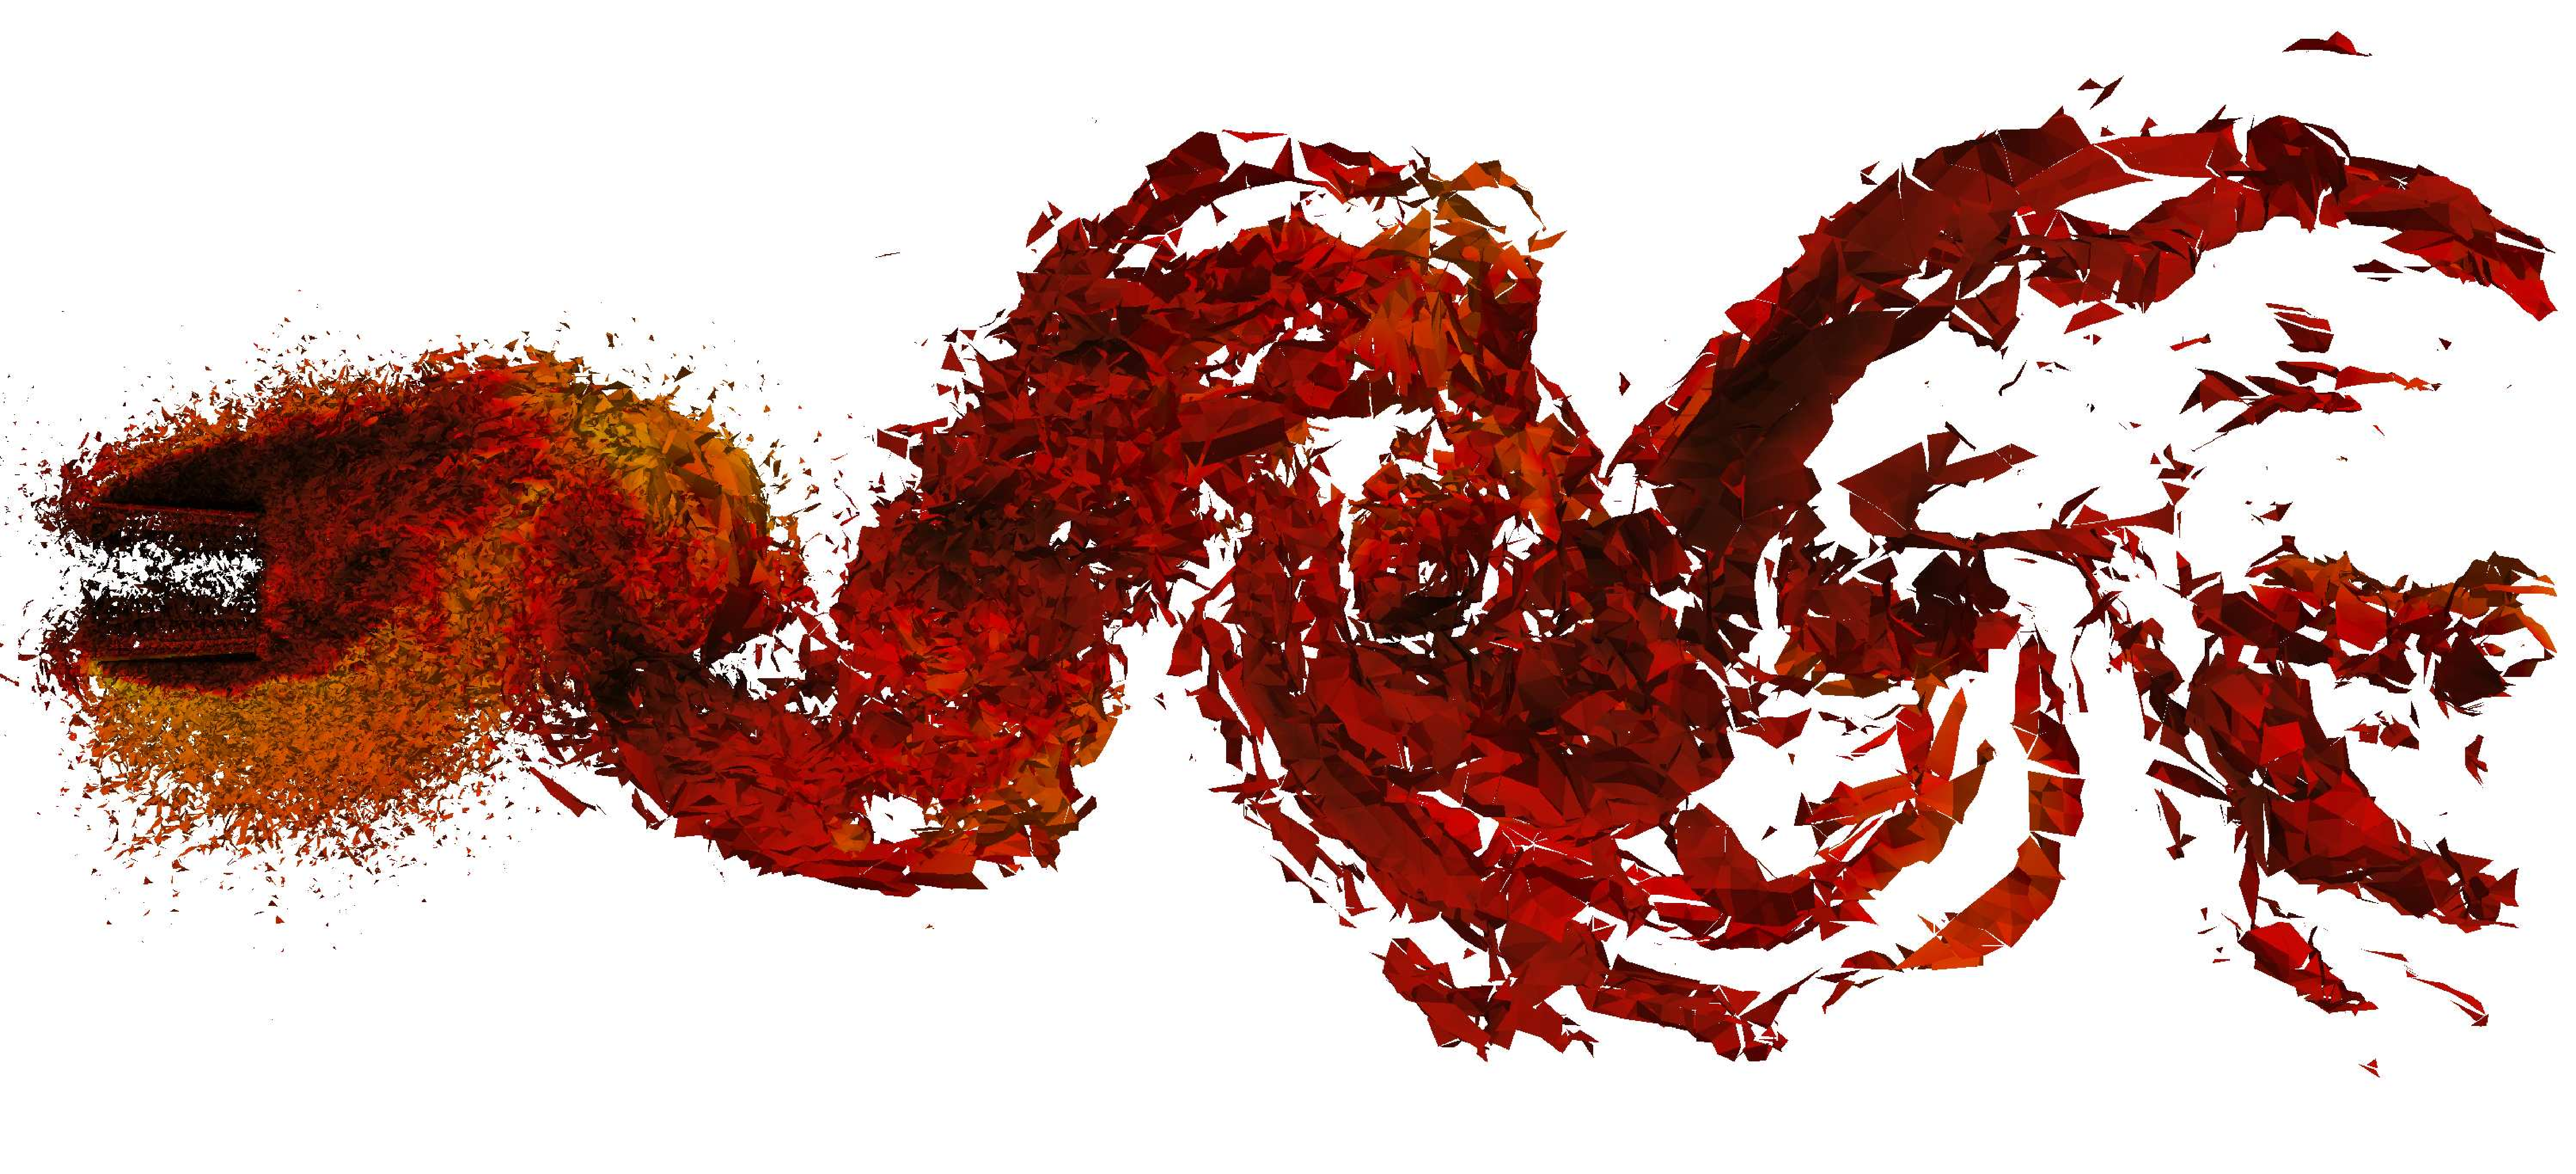
\includegraphics[width=0.9\textwidth]{sqcyl-tet-wsm-newwallfn-coarse3-qcrit-010-velomag.pdf}
\caption{Isosurface of the $q$-criterion colored by velocity magnitude showing the wake behind the square cylinder}
\label{sqcylqcrit}
\end{figure}

\begin{figure}[h]
\centering
\subfloat[Mean streamwise velocity $\langle u \rangle/u_B$]{
\includegraphics*[width=0.8\textwidth]{sqcyl-tet-wsm-newfilt-coarse-fixbc-meanu-vprofile-small.pdf}}\\
\subfloat[Mean vertical velocity $\langle v \rangle/u_B$]{
\includegraphics*[width=0.8\textwidth]{sqcyl-tet-wsm-newfilt-coarse-fixbc-meanv-vprofile-small.pdf}}\\
\subfloat[Mean Reynolds stress $\langle u'u' \rangle/u_B^2$]{
\includegraphics*[width=0.8\textwidth]{sqcyl-tet-wsm-newfilt-coarse-fixbc-meanuu-vprofile-small.pdf}}\\
\subfloat[Mean Reynolds stress $\langle u'v' \rangle/u_B^2$]{
\includegraphics*[width=0.8\textwidth]{sqcyl-tet-wsm-newfilt-coarse-fixbc-meanuv-vprofile-small.pdf}}
\caption{\small (a) Mean streamwise and vertical velocity and mean Reynolds stresses along vertical lines in the wake.
(---) current results, (- - - ) 4th order \gls{sd}+\gls{wsm} on hexahedral mesh by Lodato and Jameson~\cite{lodato2012b}, ($\circ$) \gls{ldv} experiments by Lyn et al.~\cite{lyn1994,lyn1995}.}
\label{sqcylplots}
\end{figure}



% !TEX root = ../thesis.tex
\graphicspath{{\aiaadir /figures_RANS_naca0012/}}% Set graphics path location

\subsection{NACA 0012 airfoil at 0$\degr$ angle of attack, Re = 6 million, Ma = 0.15}
In this section, the NACA 0012 airfoil is used to study the accuracy of the \gls{sa} turbulence model coupled with \gls{fr}. The NACA 0012 is commonly used as a validation case for all turbulence models and a large database of results are available at the NASA Turbulence Modeling Resource website. A $6,539$ element quad/triangle mixed mesh is used with a NACA 0012 airfoil of chord length $1.0$ and a farfield boundary $20$ chord lengths away. The results are compared with CFL3D and experimental results from Gregory \& O'Reilly~\cite{gregory1973low}.

\begin{figure}

    \subfloat[Zoomed view of the mixed element mesh near the NACA 0012 airfoil.]{\includegraphics[width = 0.5\textwidth]{NACA0012_Re6mil_mesh.eps}}
    \subfloat[X-momentum contours near the NACA 0012 airfoil]{\includegraphics[width = 0.5\textwidth]{NACA0012_Re6mil_alp0_momx.eps}}

  \caption{Turbulent flow past a NACA 0012 airfoil at \gls{re} = 6 million, \gls{ma} = 0.15, $\alpha = 0^{\circ}$ using \gls{fr} to recover 4th order accurate \gls{dg} method and the \gls{sa} turbulence model.}
  \label{RANS_naca0012}
\end{figure}

\begin{figure}
\centering
  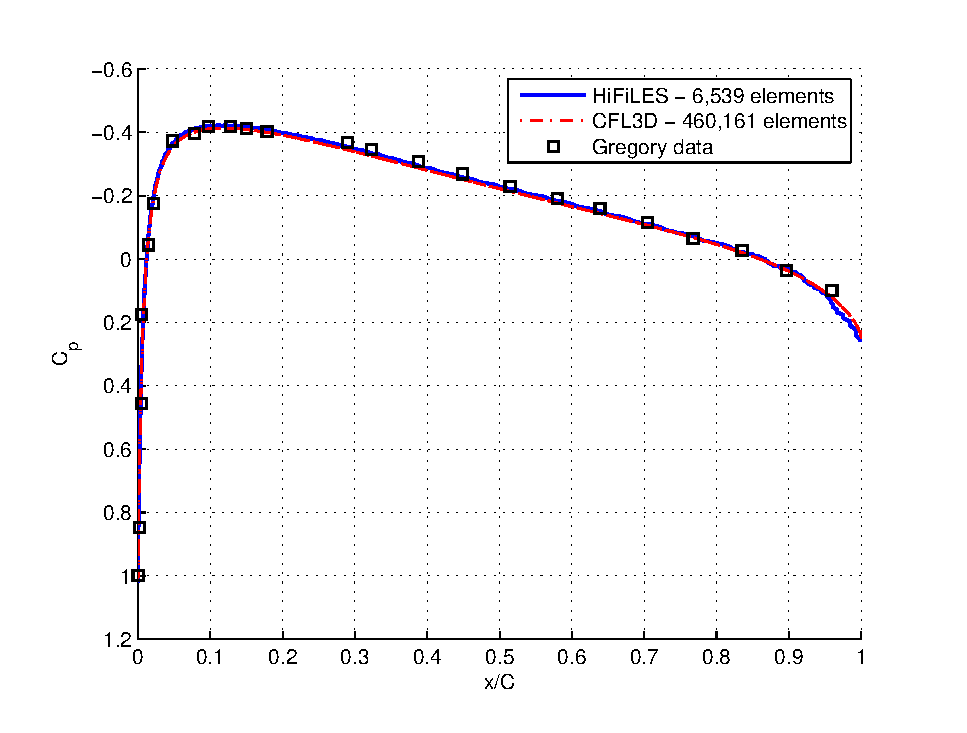
\includegraphics[width=0.48\textwidth]{cp.eps}
  \caption{Pressure coefficient on the NACA 0012 airfoil at \gls{re} = 6 million, \gls{ma} = 0.15, $\alpha = 0^{\circ}$ using \gls{fr} to recover 4th order accurate \gls{dg} method and the \gls{sa} turbulence model.}
  \label{RANS_naca0012_cp}
\end{figure}





% Note that the verification section above now has both V & V
%\section{Validation (Preliminary results)}
\label{sec:validation}
Here we follow some cases from the 2nd High-Order Workshop.

\subsection{Flat Plate}

\subsection{Circular Cylinder}
From David's thesis.



%\subsubsection{Vortex transport by uniform flow (2D)}
%\subsubsection{Transonic Ringleb Flow (2D)}
%\subsubsection{Flow over an Analytical Body of Revolution (3D)}

\subsection{RANS NACA 0012}

\subsection{SD7003 airfoil at 4$\degr$ angle of attack}
From David's thesis\cite{williams2013thesis}
\subsection{SD7003 wing section at 4$\degr$ angle of attack}
From David's thesis.
%\subsubsection{Laminar Flow around a Delta Wing}

\subsection{DNS of the Taylor-Green Vortex at Re = 1,600}

\begin{figure}
\centering
\includegraphics[height=60mm]{./figures/dissrate-hex-mesh-small.pdf} \\
\caption{LES of Tyalor-Green Vortex at Re=1,600\cite{bull2013a}}
\label{fig:setup}
\end{figure}


\subsection{DNS of Decaying Homogeneous Turbulence}
To be done by Manuel
\subsection{LES of Decaying Homogeneous Turbulence}
To be done by Manuel



% !TEX root = ./main.tex

\section{Conclusion}
\label{sec:conclusion_hf}

In this chapter, we have presented a comprehensive description, verification and validation of the \gls{hf} solver. In its first version, \gls{hf} offers to its users an optimal implementation of the \gls{fr} methodology in unstructured 3D grids using \gls{gpu}s or traditional \gls{mpi}. The implementation has been verified via \gls{mms}. The code has been tested in some difficult \gls{ns} and \gls{les} problems with very satisfactory results.

%pros:
The power of the \gls{fr} method is in its flexibility, efficiency and accuracy.
Different high-order schemes can be recovered by choosing a single parameter, allowing the numerical behavior to be fine-tuned.
%cons:
Though the use of explicit timestepping sets limits on the \gls{cfl} condition, the fact that \gls{hf} can be run on high performance multi-\gls{gpu} platforms more than compensates for this.


Despite considerable advances in the accuracy and versatility of \gls{sgs} models, current industrial \gls{cfd} codes are restricted in their ability to perform \gls{les} of turbulent flows by the use of highly dissipative second-order numerical schemes.
Therefore, in order to advance the state of the art in industrial \gls{cfd}, it is necessary to move to high-order accurate numerical methods.
The \gls{esfr} family of schemes are ideal for resolving turbulent flows due to low numerical dissipation and high-order accurate representation of solution gradients at the small scales.
Advanced subgrid-scale models have been implemented in \gls{hf} for all element types, enabling simulation of turbulent flows over complex geometry.
The development of the first high-order accurate solver for unstructured meshes incorporating \gls{les} modeling capabilities represents a significant step towards tackling challenging compressible turbulent flow problems of practical interest.
Future additions will include optimization of the \gls{esfr} schemes for turbulence resolution, moving mesh capabilities,  multigrid convergence acceleration, and advanced turbulence modeling.